
%----------------------------------------------------------------------------------------
%	SECTION 5
%----------------------------------------------------------------------------------------

\section{Sunamp, July - August 2018} \label{sec:sunamp}


\subsection*{The Company}

% copied and pasted from Susan's emails %

Sunamp designs and produces super-compact heat batteries which store available energy as heat and release it when it is required, thus overcoming the intermittent nature of many other renewable energy sources.
The technology is based on phase change materials (PCMs) to provide a clean, efficient and cost-effective heat energy storage solution.


Working with multiple energy sources including solar and heat pumps, the company’s UniQ range of heat batteries has the potential to make conventional hot water cylinders obsolete and delivers cascades of hot water and highly responsive space heating with proven savings of up to 75\% on utility bills.
The technology offers limitless scalability for residential, commercial or industrial projects.


% % % % % % % % % %


%Sunamp is a newly established business that specialises in the research, production and sales of heat batteries that are based on phase change materials (PCMs).
The PCMs, developed and manufactured by Sunamp, are non-toxic, non-flammable, eco-friendly and patented in the UK and China, with patents pending in other countries \citep{SunampAutomotive}.
The PCMs operate at different temperatures, allowing the storage of heat (up to 1000$^{\circ}$C) or coolth (less than 0$^{\circ}$C) (see Figure~\ref{pcm_temp_range}).
Currently, the company's main markets are buildings, where their heat batteries can generate hot water and space heating, and automobiles, where their heat batteries can refrigerate transported goods (for example).

\begin{figure}[htbp]
	\centering
	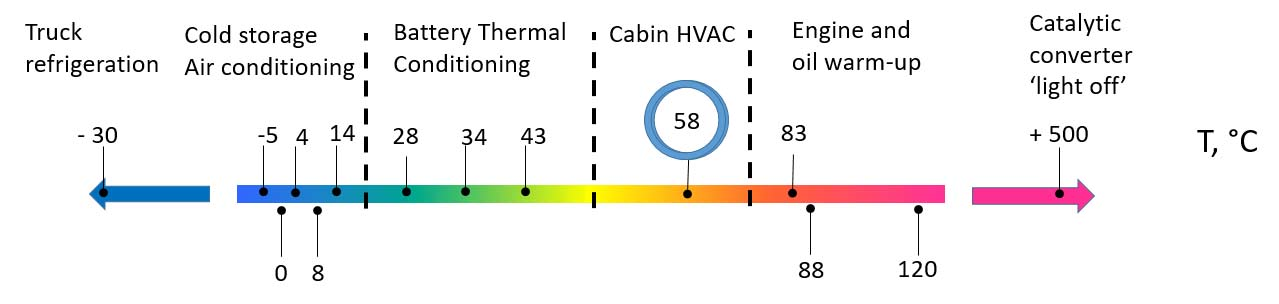
\includegraphics[width=\textwidth]{figures/temperature-range-of-PCMs.jpg}
	\rule{\textwidth}{0.5pt} % use line???
	\caption{The temperature range of Sunamp's PCMs in degrees Celsius \citep{SunampAutomotive}.}
	\label{pcm_temp_range}
\end{figure}


Sunamp was founded by Andrew Bissell, who is the chief executive officer (CEO).
In Macmerry, East Lothian, they have an office building which features a research and development (R\&D) workshop and materials laboratory on the ground floor and an open-plan office on the first floor.
They also have a factory across the road where they have additional test facilities but primarily do large-scale manufacturing %and packaging 
of heat batteries.
Sunamp employs 32 people: 22 office-based, six in the factory, three based on the road and one based in Zurich, where Sunamp has a small satellite office.





%%%%%%%%%%%%%%%%%%%%%%%%%%%
\subsection*{Their Products}

\begin{wrapfigure}{r}{0.3\textwidth}
	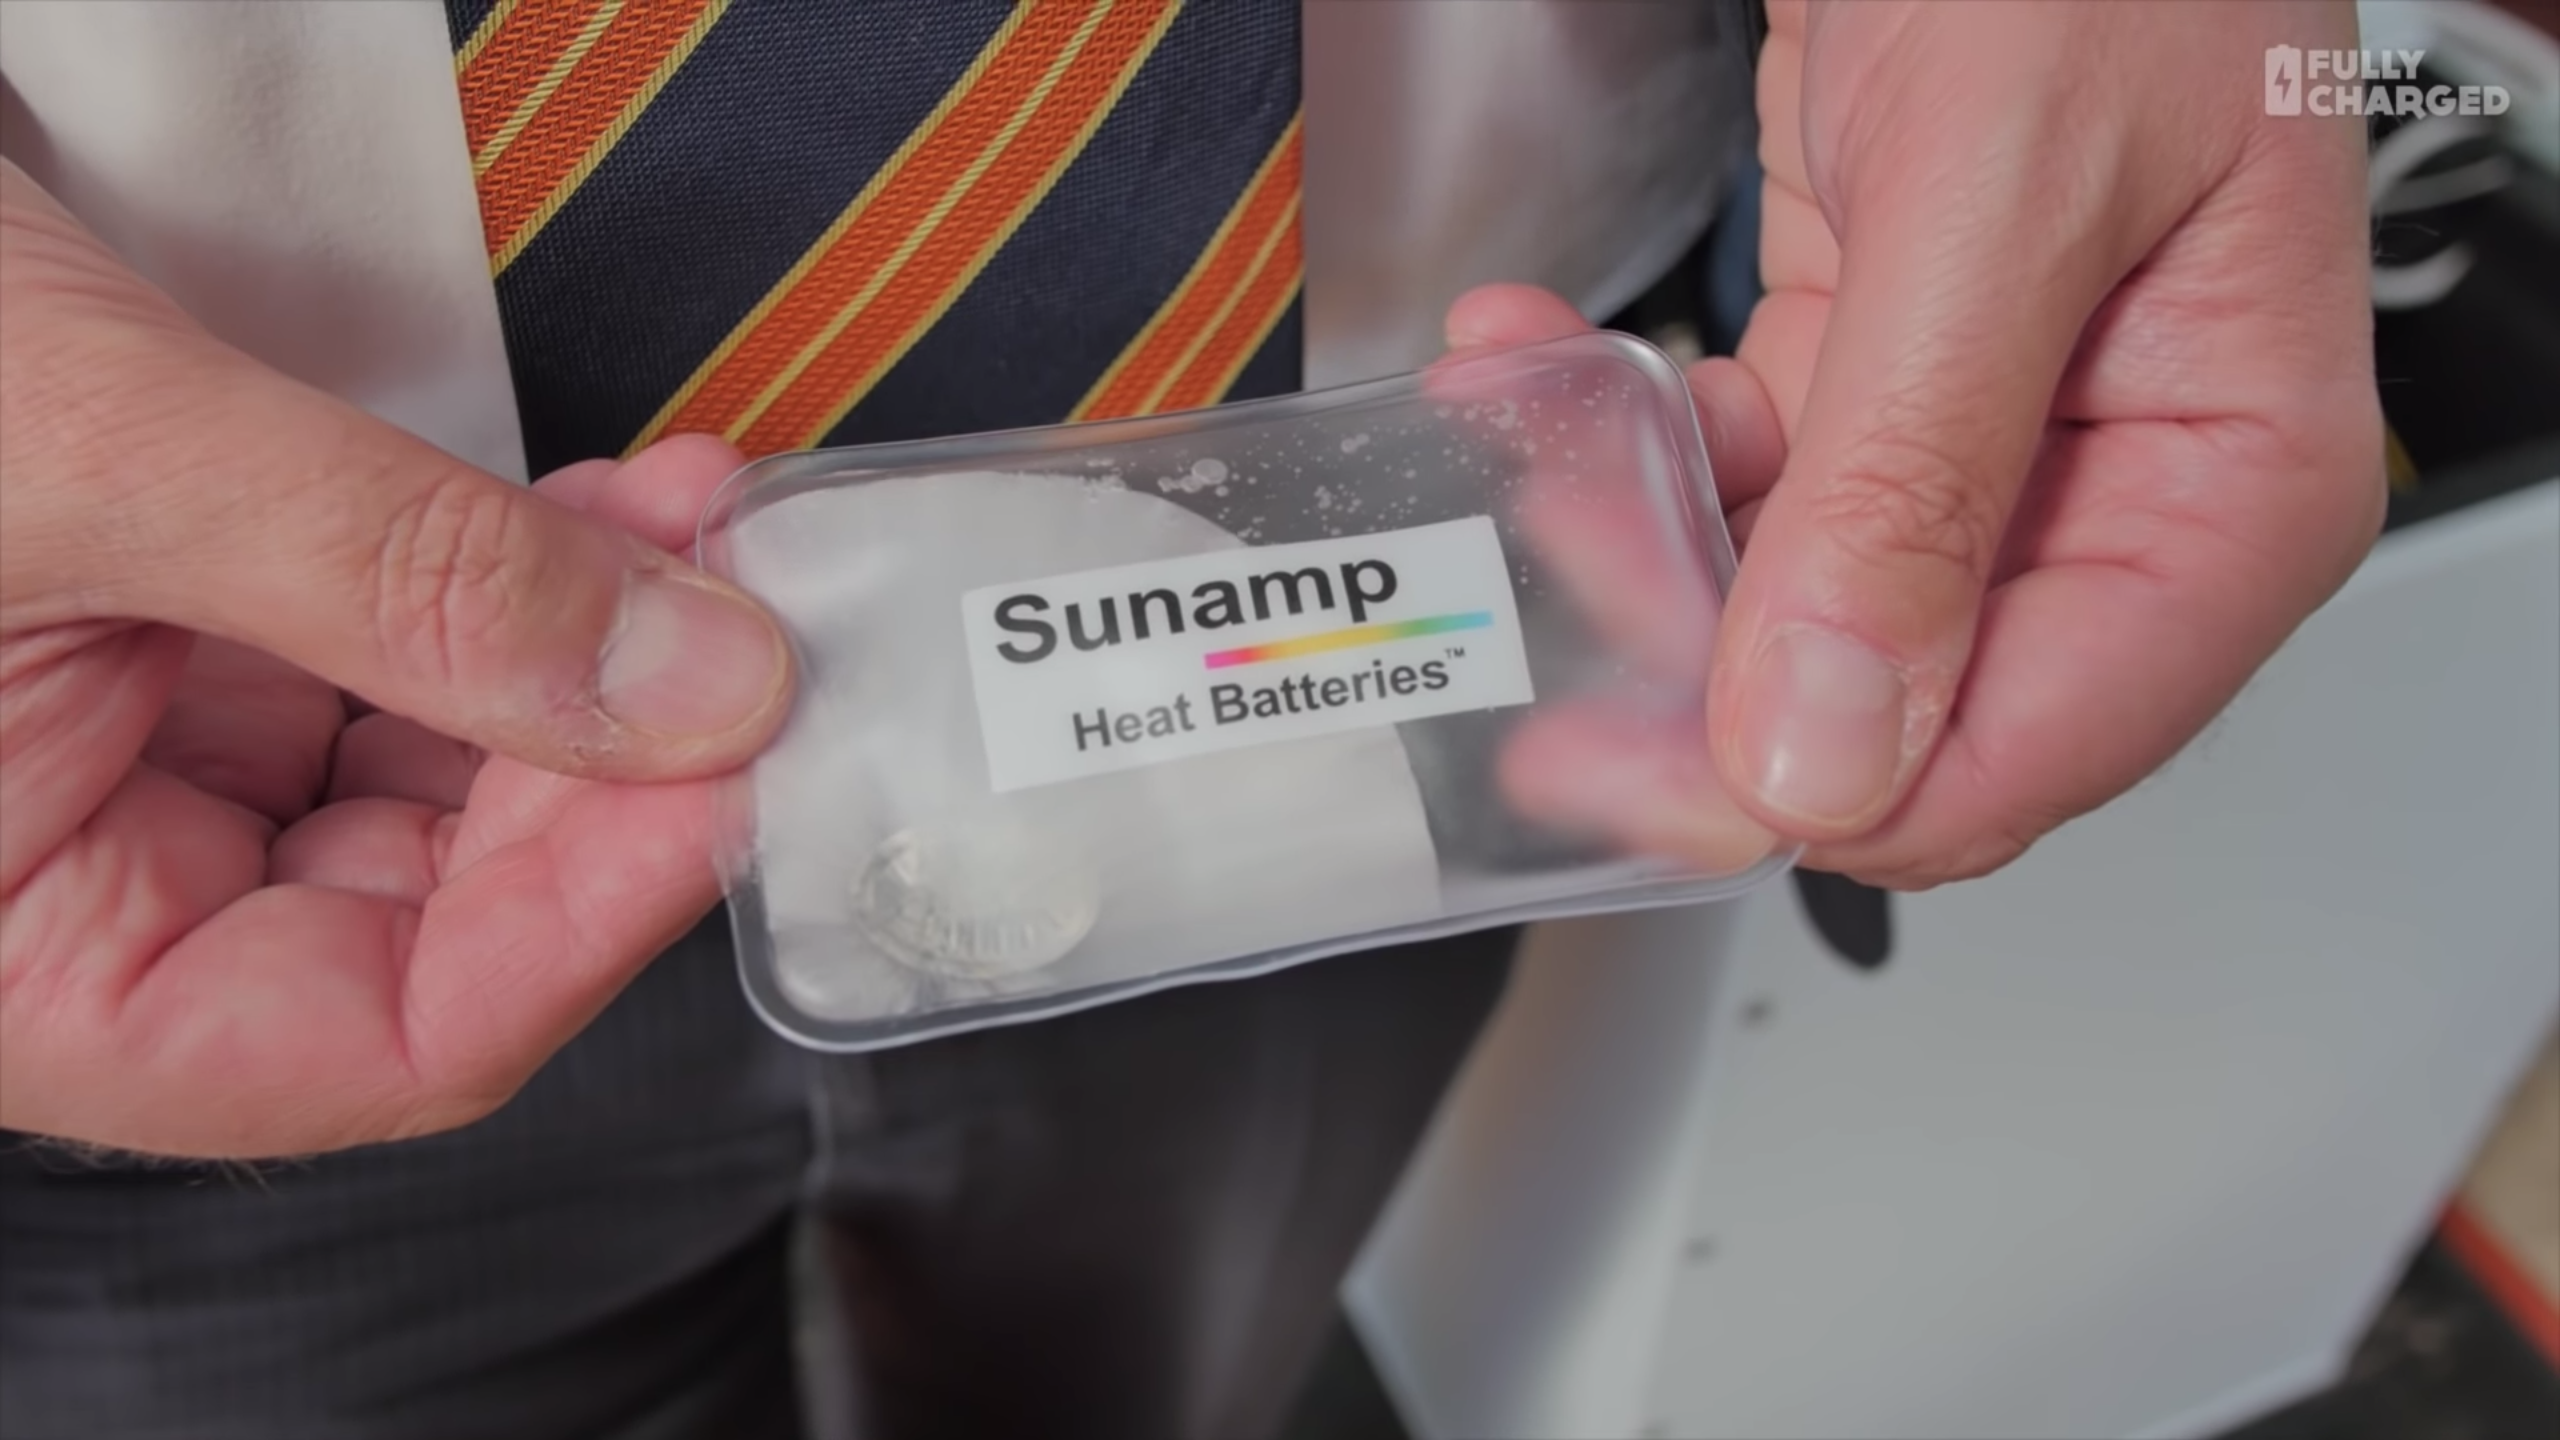
\includegraphics[width=0.3\textwidth]{figures/sunamp-hand-warmer.png}
	\rule{0.3\textwidth}{0.5pt} % use line???
	\caption{A crystallising hand warmer \citep{FullyCharged}.}
	\label{fig:handwarmer}
\end{wrapfigure}

If you have ever gone camping, you might have come across crystallisation-type reusable hand warmers (pictured in Figure~\ref{fig:handwarmer}).
Such hand warmers are filled with a PCM called sodium acetate and contain a little metal disk.
The sodium acetate is liquid at room temperature.
When you bend the metal disk, the sodium acetate gradually crystallises and releases heat 
(see a video of the crystallisation process here: 
\url{https://upload.wikimedia.org/wikipedia/commons/0/09/Hand_warmer_activation.webm} \citep{HandWarmerActivation}).
The pack becomes completely solid and continues to release heat for a while.
The hand warmer is reusable because you can turn the sodium acetate back into a liquid by immersing the pack in boiling water for about ten to 15 minutes.

The principle that makes hand warmers work is \emph{latent heat}.
Latent heat is the thermal energy required to change the phase of a substance (e.g. from a solid to a liquid, or a liquid to a gas) without it changing temperature (see Figure~\ref{fig:latentheat}).
Latent heat can be thought of as the energy required to make or break the molecular bonds within a substance, thereby changing its state.


\begin{figure}[htbp]
	\centering
	\begin{subfigure}{.49\textwidth}
		\centering
		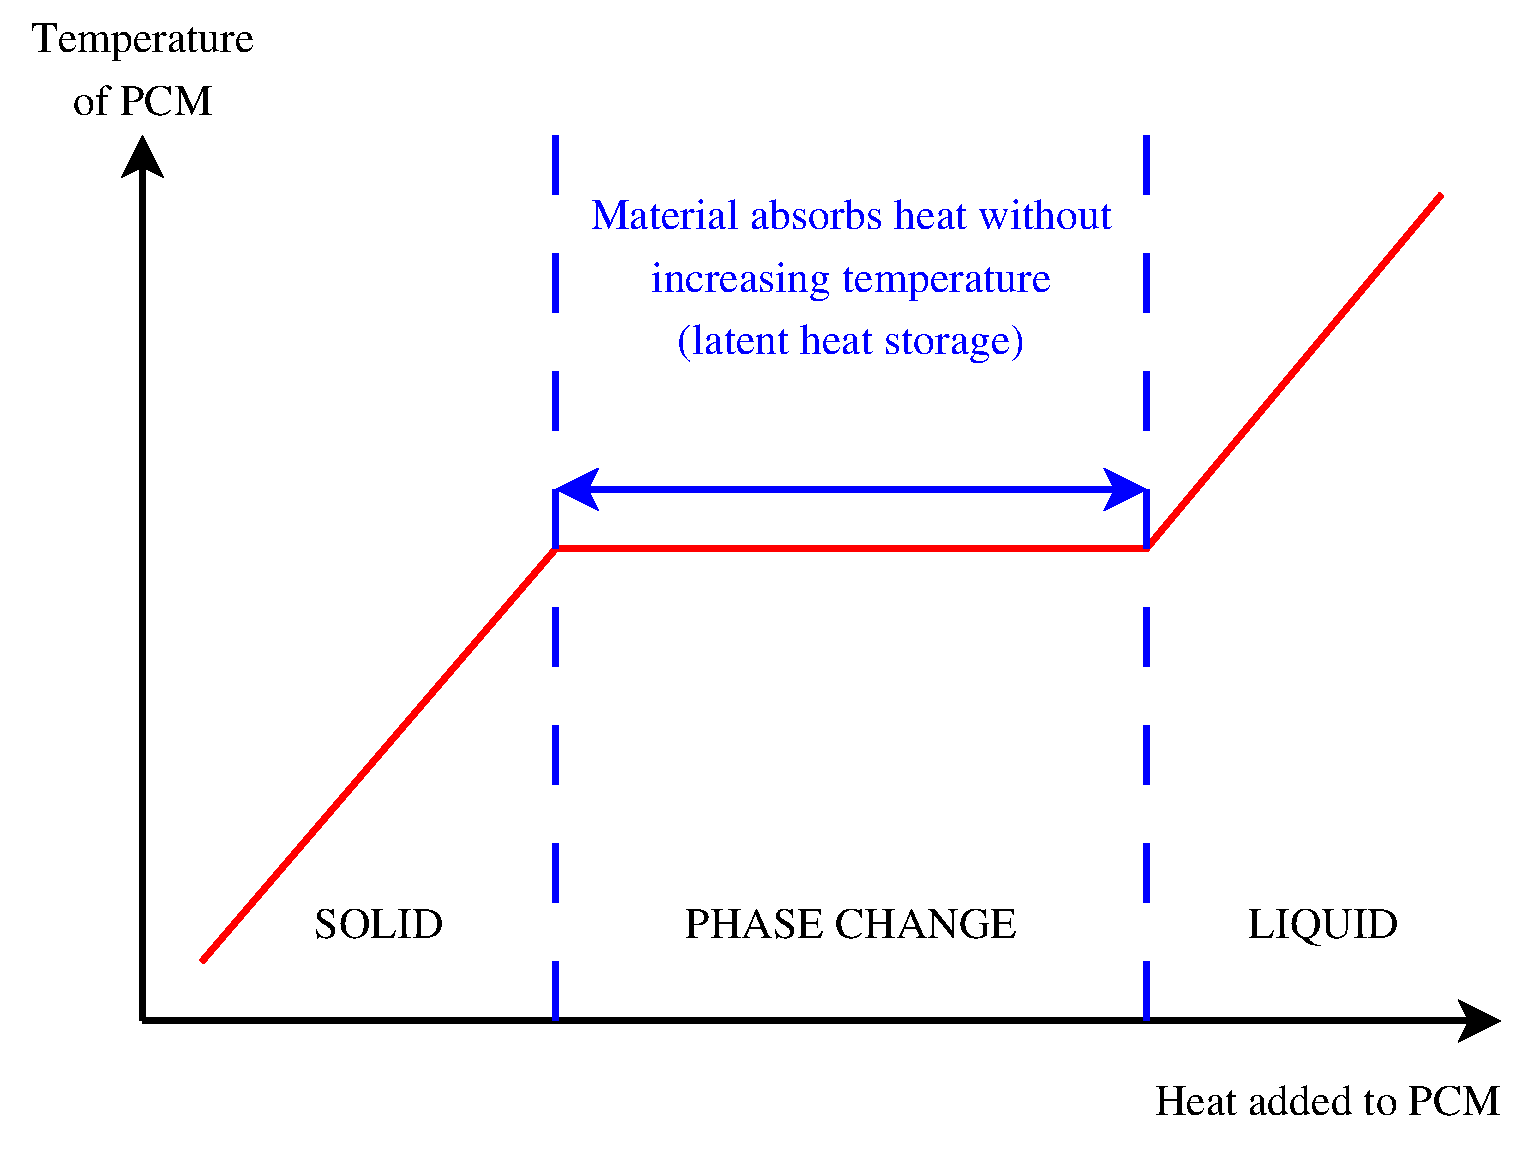
\includegraphics[width=\textwidth]{figures/LatentHeatStorage.eps}
		%          \rule{\textwidth}{0.5pt} % use line???
		\caption{Latent heat storage}
		\label{fig:latentheatstorage}
	\end{subfigure}
	\begin{subfigure}{.47\textwidth}
		\centering
		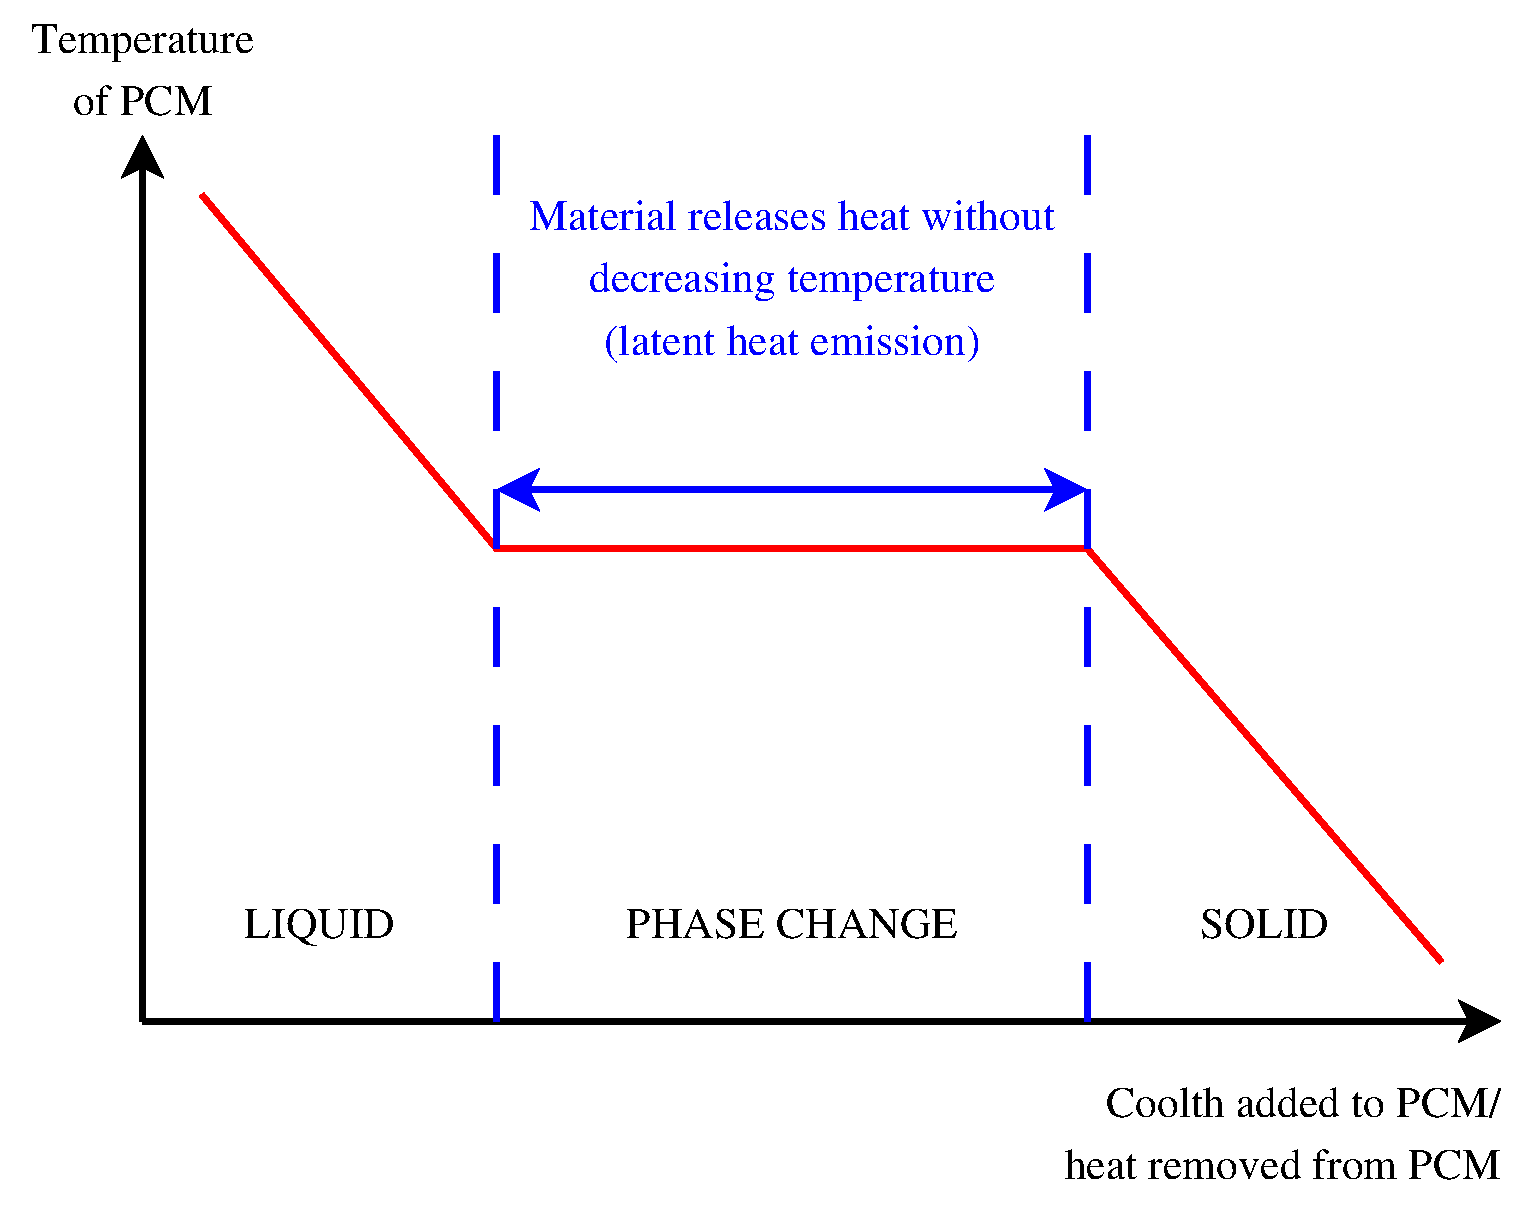
\includegraphics[width=\textwidth]{figures/LatentHeatEmission.eps}
		%          \rule{\textwidth}{0.5pt} % use line???
		\caption{Latent heat emission}
		\label{fig:latentheatemission}
	\end{subfigure}
	\rule{\textwidth}{0.5pt} % use line???
	\caption[Graphical representations of latent heat.]{Graphical representations of latent heat (slightly adapted from \EnBldgsTitle \space lecture slides \citep{jenkins}).}
	\label{fig:latentheat}
\end{figure}


%For example, take a PCM that melts at 58$^{\circ}$C.
Water is an example of a PCM.
%Water freezes at 0$^{\circ}$C, and in reverse, ice melts at 0$^{\circ}$C.
When you put water in a cold environment, like a freezer, it exchanges heat with the environment: the water loses latent heat and becomes solid ice at 0$^{\circ}$C, and the environment gains heat, becoming somewhat warmer.
When you put the solid ice in a warm environment, the reverse happens: the ice gains latent heat and becomes liquid water at 0$^{\circ}$C, and the environment loses heat, becoming somewhat cooler.
%When you put ice in a warm environment, it exchanges heat with the environment: the ice gains latent heat and becomes liquid water at 0$^{\circ}$C, and the environment loses heat, becoming somewhat cooler.
%When you put the liquid water back in a cold environment such as a freezer, the reverse happens: the water loses latent heat and becomes solid ice at 0$^{\circ}$C, and the environment gains heat, becoming somewhat warmer.

%Sunamp's heat batteries are ``scaled up" versions of crystallisation-type hand warmers.
%They charge (i.e. absorb heat) when heat is added to the battery, e.g. via piped hot water running through the battery or via an electrical heating element inside the battery.
%They then discharge (i.e. release heat) when piped cold water runs through the battery, thereby exchanging heat with the water.
%The hot water that is discharged from the battery can be used for space heating and hot water purposes in buildings.


\begin{figure}[htbp]
	\centering
	\begin{subfigure}{.24\textwidth}
		\centering
		
\includegraphics[width=\textwidth]{figures/sunamp-uniq-3.png}
		%          \rule{\textwidth}{0.5pt} % use line???
		\caption{UniQ 3\\
			(3.5 kWh)}
		\label{fig:uniq3}
	\end{subfigure}
	\begin{subfigure}{.24\textwidth}
		\centering
		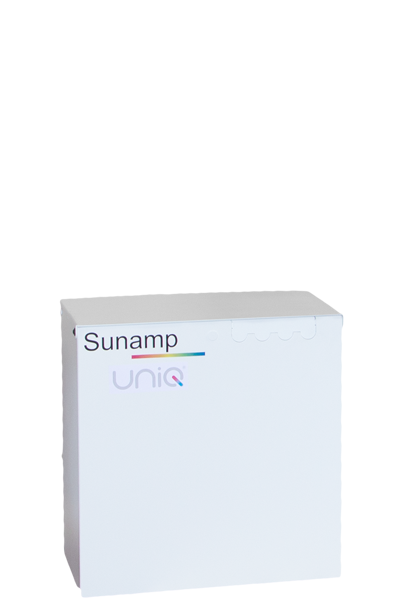
\includegraphics[width=\textwidth]{figures/sunamp-uniq-6.png}
		%          \rule{\textwidth}{0.5pt} % use line???
		\caption{UniQ 6\\
			(7.0 kWh)}
		\label{fig:uniq6}
	\end{subfigure}
	\begin{subfigure}{.24\textwidth}
		\centering
		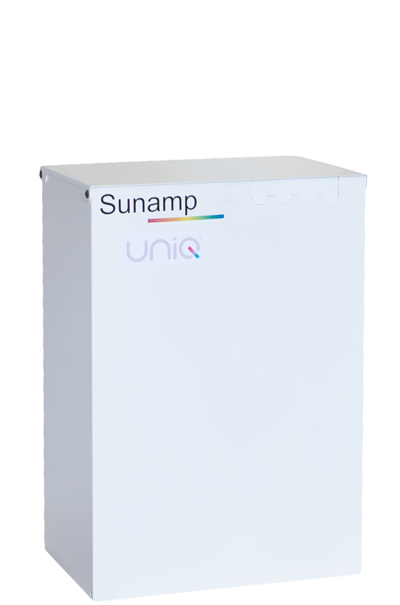
\includegraphics[width=\textwidth]{figures/sunamp-uniq-9.png}
		%          \rule{\textwidth}{0.5pt} % use line???
		\caption{UniQ 9\\
			(10.5 kWh)}
		\label{fig:uniq9}
	\end{subfigure}
	\begin{subfigure}{.24\textwidth}
		\centering
		
\includegraphics[width=\textwidth]{figures/sunamp-uniq-12.png}
		%          \rule{\textwidth}{0.5pt} % use line???
		\caption{UniQ 12\\
			(14 kWh)}
		\label{fig:uniq12}
	\end{subfigure}
	\rule{\textwidth}{0.5pt} % use line???
	\caption{Sunamp's UniQ heat battery range and nominal heat storage capacities in kWh \citep{SunampHomepage}.}
	\label{fig:uniq_range}
\end{figure}


Sunamp's latest range of heat batteries is called \emph{UniQ} (see Figure~\ref{fig:uniq_range}).
Why?
\emph{Uni} because it is the ``one and only energy storage solution you need for" \emph{Q}, the ``engineering symbol for Heat Energy" \citep{UniQ_Leaflet}.
The UniQ batteries are ``scaled up" versions of crystallisation-type hand warmers.
There are two series of UniQ batteries: standard batteries and e-batteries.
Broadly speaking, a standard UniQ battery consists of a highly insulated box which contains a finned-tube heat exchanger and a PCM which fills the space around the heat exchanger (see cross-section in Figure~\ref{fig:uniq_cross-section}).
The tubes of the heat exchanger protrude from the box, allowing pipe connections to serve as hot and cold water inlets to the battery, as well as hot water and space heating outlets from the battery.
A UniQ e-battery has a similar construction, except it also contains an electrical heating element (see Figure~\ref{fig:euniq_cross-section}).
A battery charges (i.e. its PCM absorbs heat) when heat is added to it, e.g. via piped hot water running through a standard battery or by switching on the electrical heating element inside an e-battery.
A battery then discharges (i.e. its PCM releases heat) when piped cold water runs through it, the warm PCM thereby exchanging heat with the cold water.
The hot water that is discharged from the battery can be used for space heating and hot water purposes in buildings.


\begin{figure}[htbp]
	\centering
	\begin{subfigure}{.48\textwidth}
		\centering
		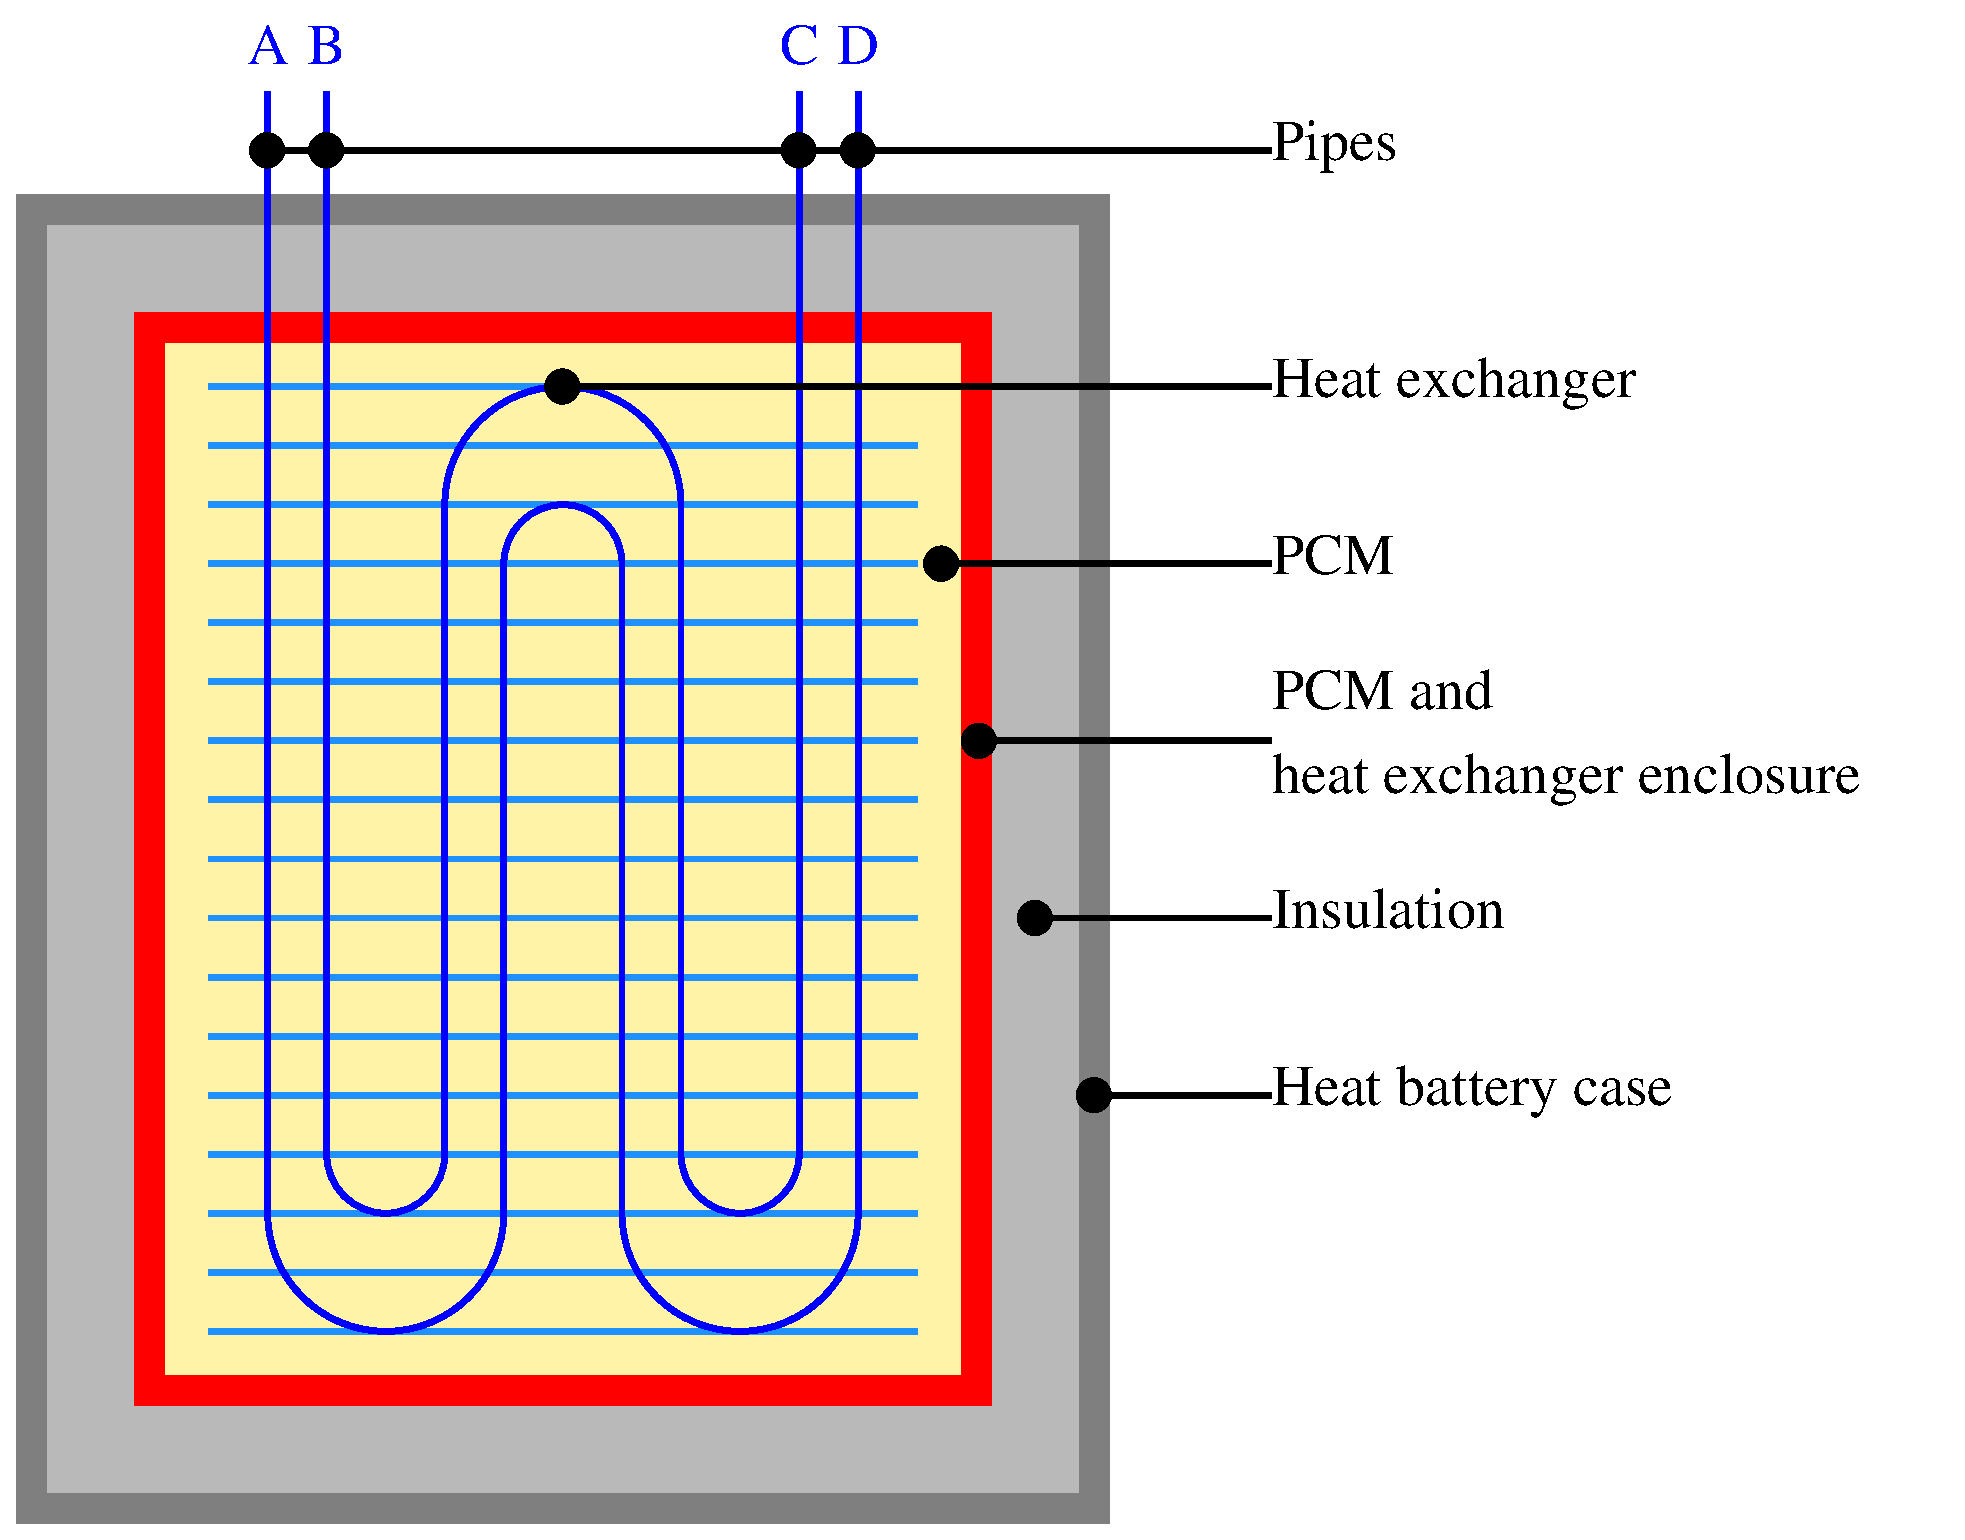
\includegraphics[width=\textwidth]{figures/UniQ_std_cross-section.eps}
		%          \rule{\textwidth}{0.5pt} % use line???
		\caption{Standard UniQ battery}
		\label{fig:uniq_cross-section}
	\end{subfigure}
	\begin{subfigure}{.48\textwidth}
		\centering
		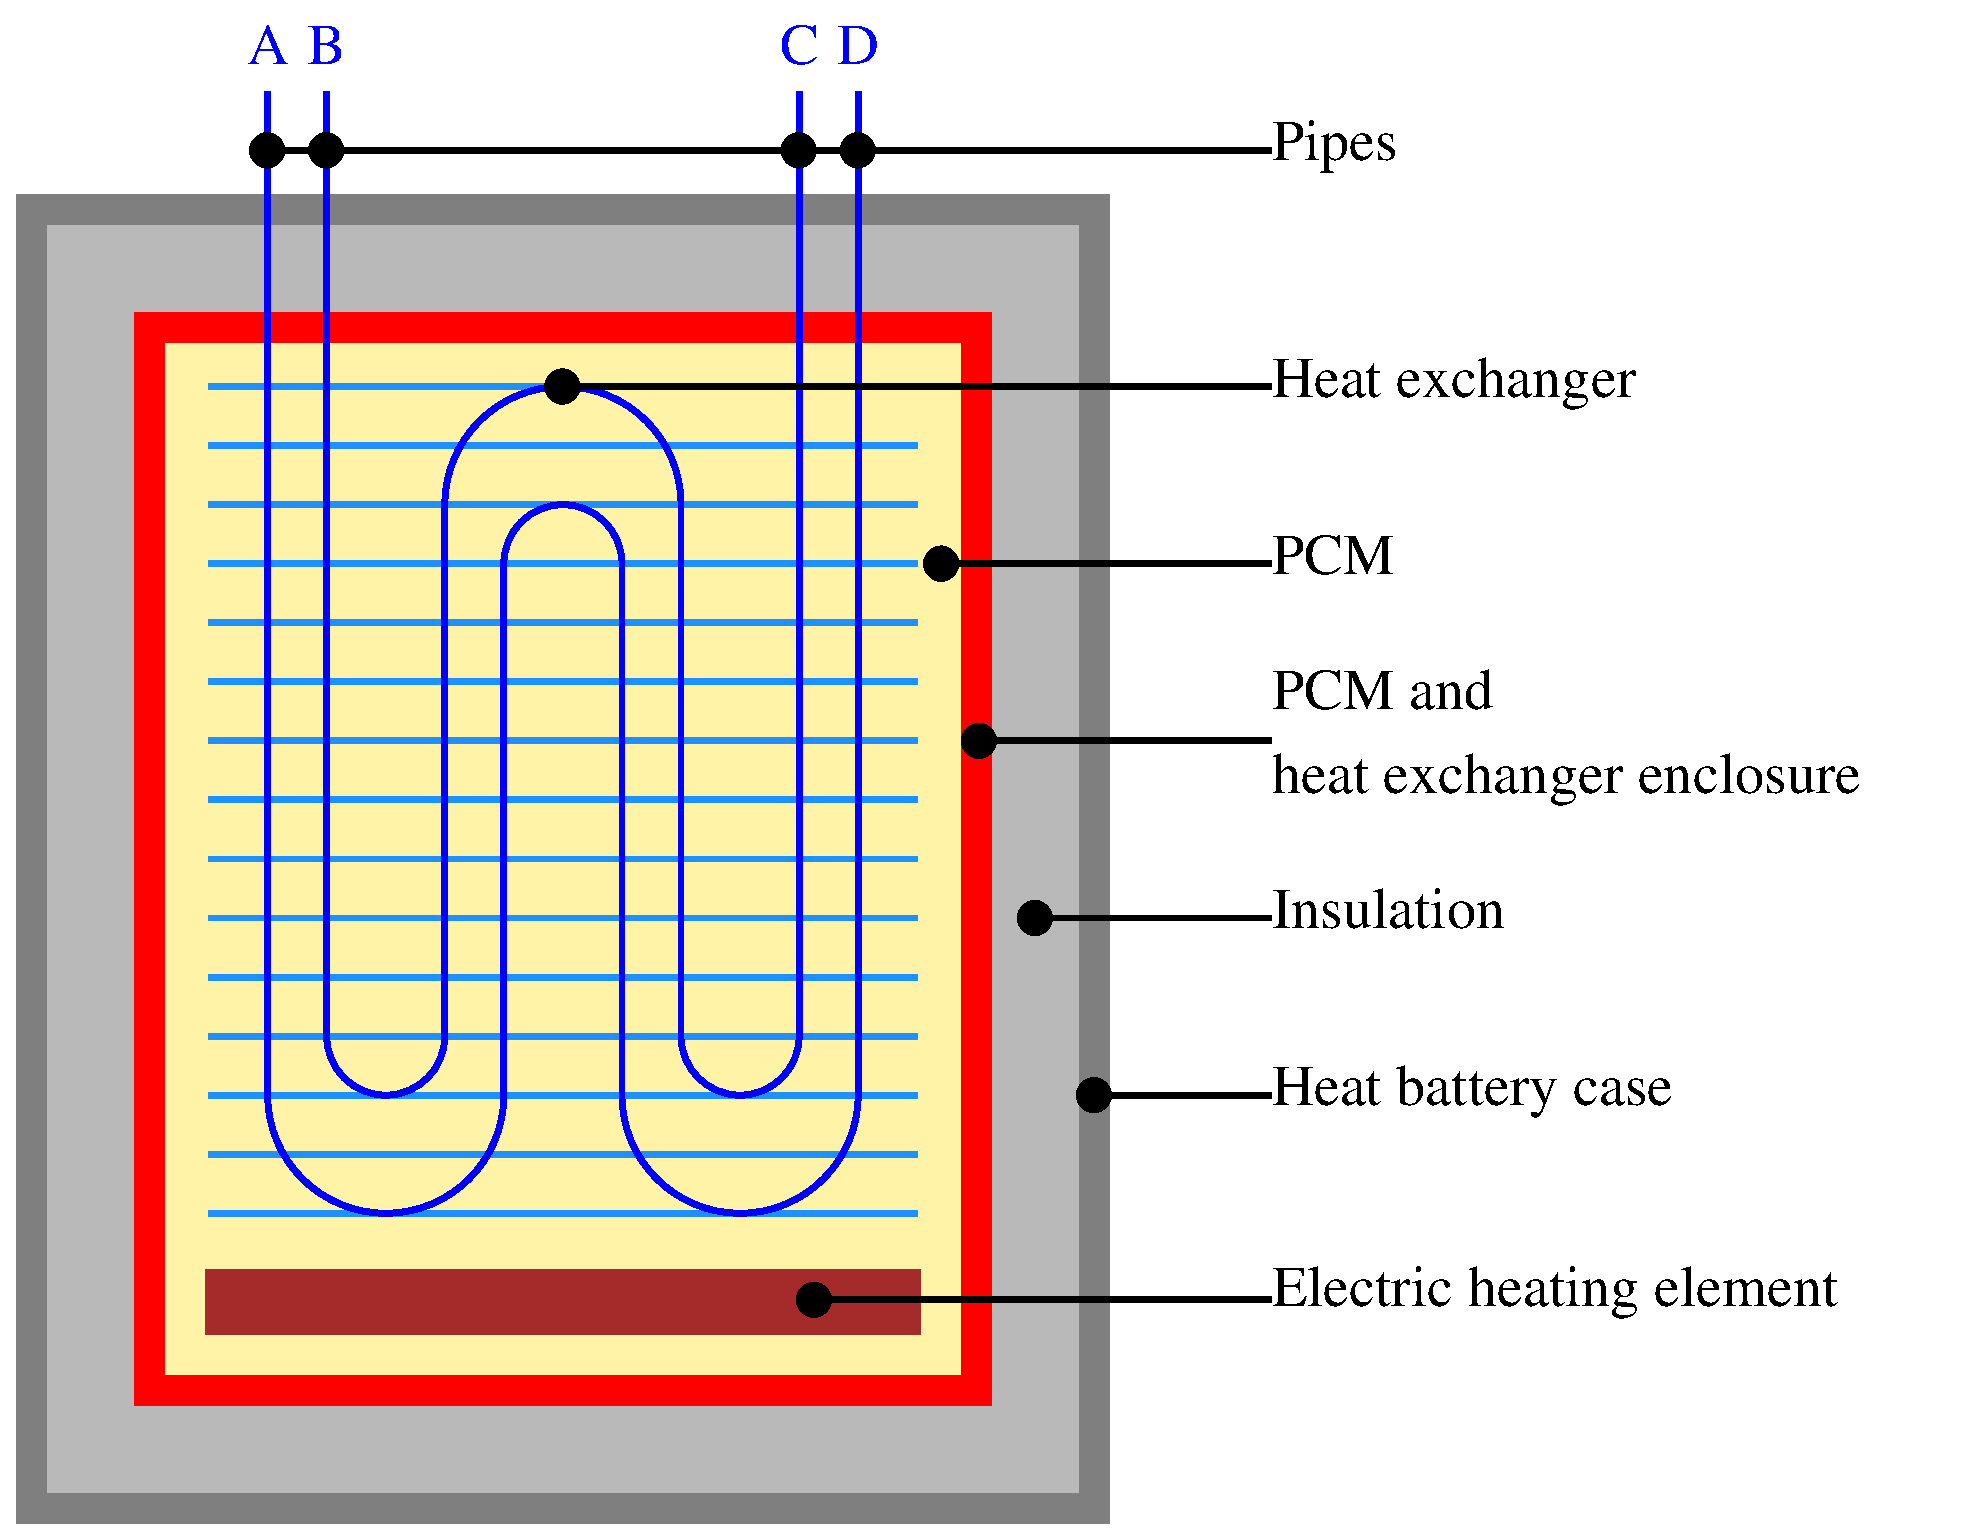
\includegraphics[width=\textwidth]{figures/eUniQ_cross-section.eps}
		%          \rule{\textwidth}{0.5pt} % use line???
		\caption{UniQ e-battery}
		\label{fig:euniq_cross-section}
	\end{subfigure}
	\rule{\textwidth}{0.5pt} % use line???
	\caption{Cross-sections of Sunamp's UniQ batteries.}
	\label{fig:cross-sections}
\end{figure}


%%%%%%%%%%%%%%%%%%%%%%%%%%%
\newpage
\subsection*{Why Heat Batteries?}

\begin{wrapfigure}{r}{0.4\textwidth}
	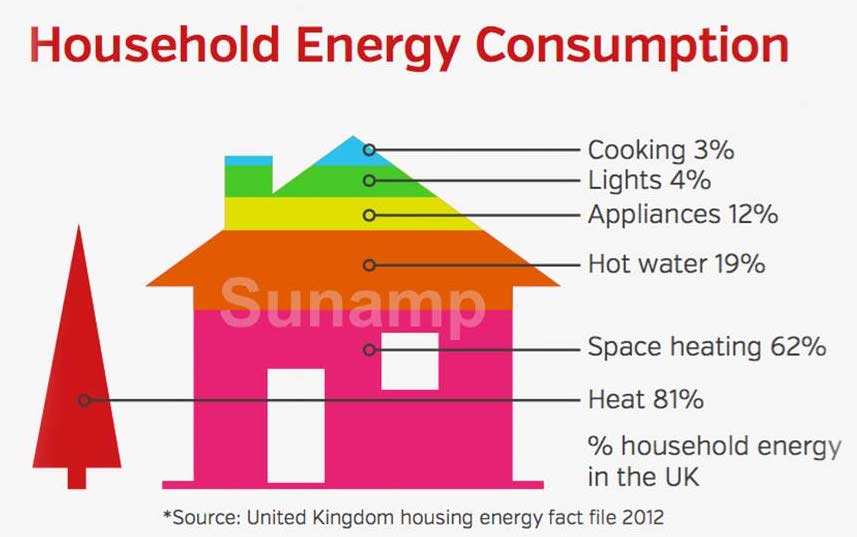
\includegraphics[width=0.4\textwidth]{figures/household-energy-consumption.jpg}
	\rule{0.4\textwidth}{0.5pt} % use line???
	\caption{Typical energy consumption of a UK home \citep{SunampResidential}.}
	\label{fig:domestic-energy}
\end{wrapfigure}

Electric batteries like the Tesla Powerwall have gained a lot of media attention recently for being able to store renewable electricity and shift demand etc.
However, in the UK (and probably other countries with a similar climate), over 80\% of domestic energy is used to generate heat for space heating and hot water (see Figure~\ref{fig:domestic-energy}).
Considering that the majority of UK households generate heat from natural gas, and some from fossil fuelled electricity, that causes a large carbon footprint.
Moreover, the current heat storage solutions are not as effective as they could be.
For example, in my flat, I have a direct hot water cylinder which turns on early every morning so that I have hot water as soon as I wake up.
But by the evening, the water is lukewarm or cold and, if I require any more hot water, I need to use more electricity to boost the hot water cylinder.
The poor heat storage capacity of my cylinder is probably due to its poor insulation, but perhaps also due to the relatively low heat capacity of water.
For a sustainable future, we need to be smarter about the way we generate and use heat, which is something we are evidently highly dependent on.




Sunamp’s UniQ heat batteries offer a smart solution to sustainable heat generation and consumption.
%Due to the high specific heat capacity of their PCMs, problems such as me re-boosting my hot water cylinder can be avoided.
%OR 
Due to the high heat capacity of their PCMs\footnote{
	I do not know the heat capacity of Sunamp's PCMs, but to get an idea, the heat capacity of sodium acetate can be as high as 229 $J/mol \cdot K$ \citep{Csodiumacetate} whereas that of water is 69.95 $J/mol \cdot K$ \citep{Cwater} according to the National Institute of Standards and Technology (NIST).
} and the low heat losses of their batteries, an excessive amount of energy does not need to be used to generate or store heat (cf. my aforementioned hot water cylinder example).
Moreover, their heat batteries can be charged by any energy source, including renewable and/ or environmentally friendly technologies such as PVs and heat pumps. %, which are energy generation solutions for a sustainable future.
%Furthermore, with thoughts to electrify heat in the UK (as grid electricity gradually becomes decarbonised), 
UniQ e-batteries also allow for demand-side management (DSM) which helps with grid balancing, e.g. by shifting electricity demands from peak periods, thus reducing the strain on the national electricity supply system (see Figure~\ref{fig:DSM}).
DSM might become an increasingly important strategy since there have been thoughts to electrify heat in the UK as grid electricity gradually becomes decarbonised.




\begin{wrapfigure}[3]{r}{0.2\textwidth}
	\centering
	\begin{subfigure}{.2\textwidth}
		\centering
		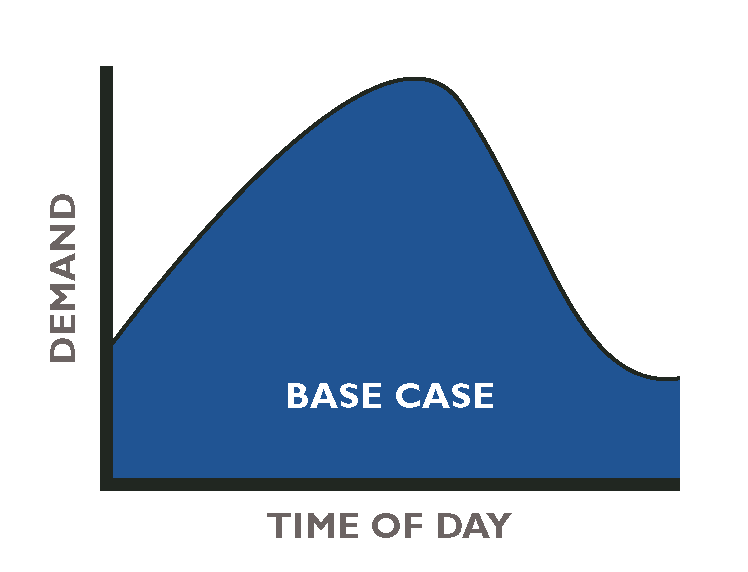
\includegraphics[width=\textwidth]{figures/DSM-base.png}
		%          \rule{\textwidth}{0.5pt} % use line???
		%\caption{Latent heat storage}
		%\label{fig:latentheatstorage}
	\end{subfigure}
	\begin{subfigure}{.2\textwidth}
		\centering
		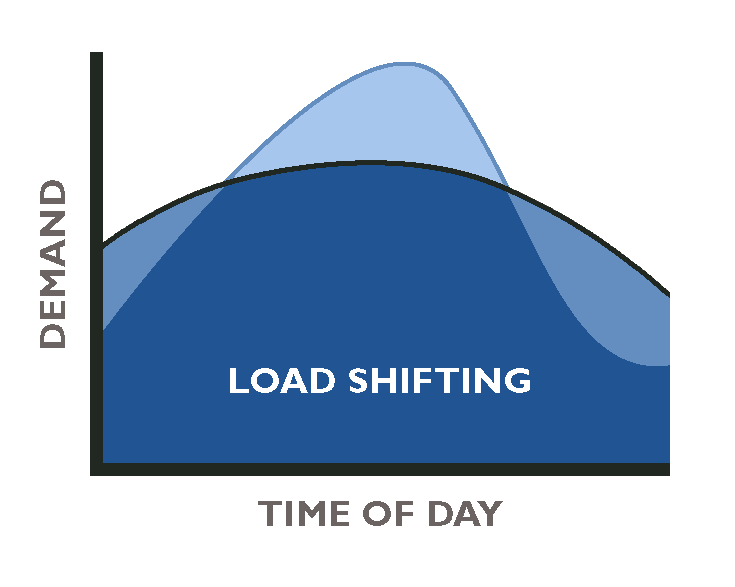
\includegraphics[width=\textwidth]{figures/DSM-load-shift.png}
		%          \rule{\textwidth}{0.5pt} % use line???
		%\caption{Latent heat emission}
		%\label{fig:latentheatemission}
	\end{subfigure}
	\rule{0.2\textwidth}{0.5pt} % use line???
	\caption[Load shifting, an example of DSM.]{Load shifting, an example of DSM \citep{USAID}).}
	\label{fig:DSM}
\end{wrapfigure}

Other key features of UniQ batteries include:
\begin{itemize}
	\item Instant hot water at mains pressure
	\item Rapid warm-up of your heating system, e.g. radiators
	\item Significantly reduced legionella risk, since there is hardly any risk of water stagnating or being between 20$^{\circ}$C and 45$^{\circ}$C inside the battery \citep{HSE_legionella}
	\item Compact, between two and four times smaller than the equivalent hot water cylinders
	\item Reliable, with a lifespan of at least 50 years
	\item Modular: the batteries can easily be combined to increase heat storage
	\item You can save money by charging your e-battery during off-peak periods with variable rate electricity tariffs, e.g. Economy 10
\end{itemize}



%%%%%%%%%%%%%%%%%%%%%%%%%%%

\subsection*{Description of Work Experience}

\begin{wrapfigure}{r}{0.4\textwidth}
	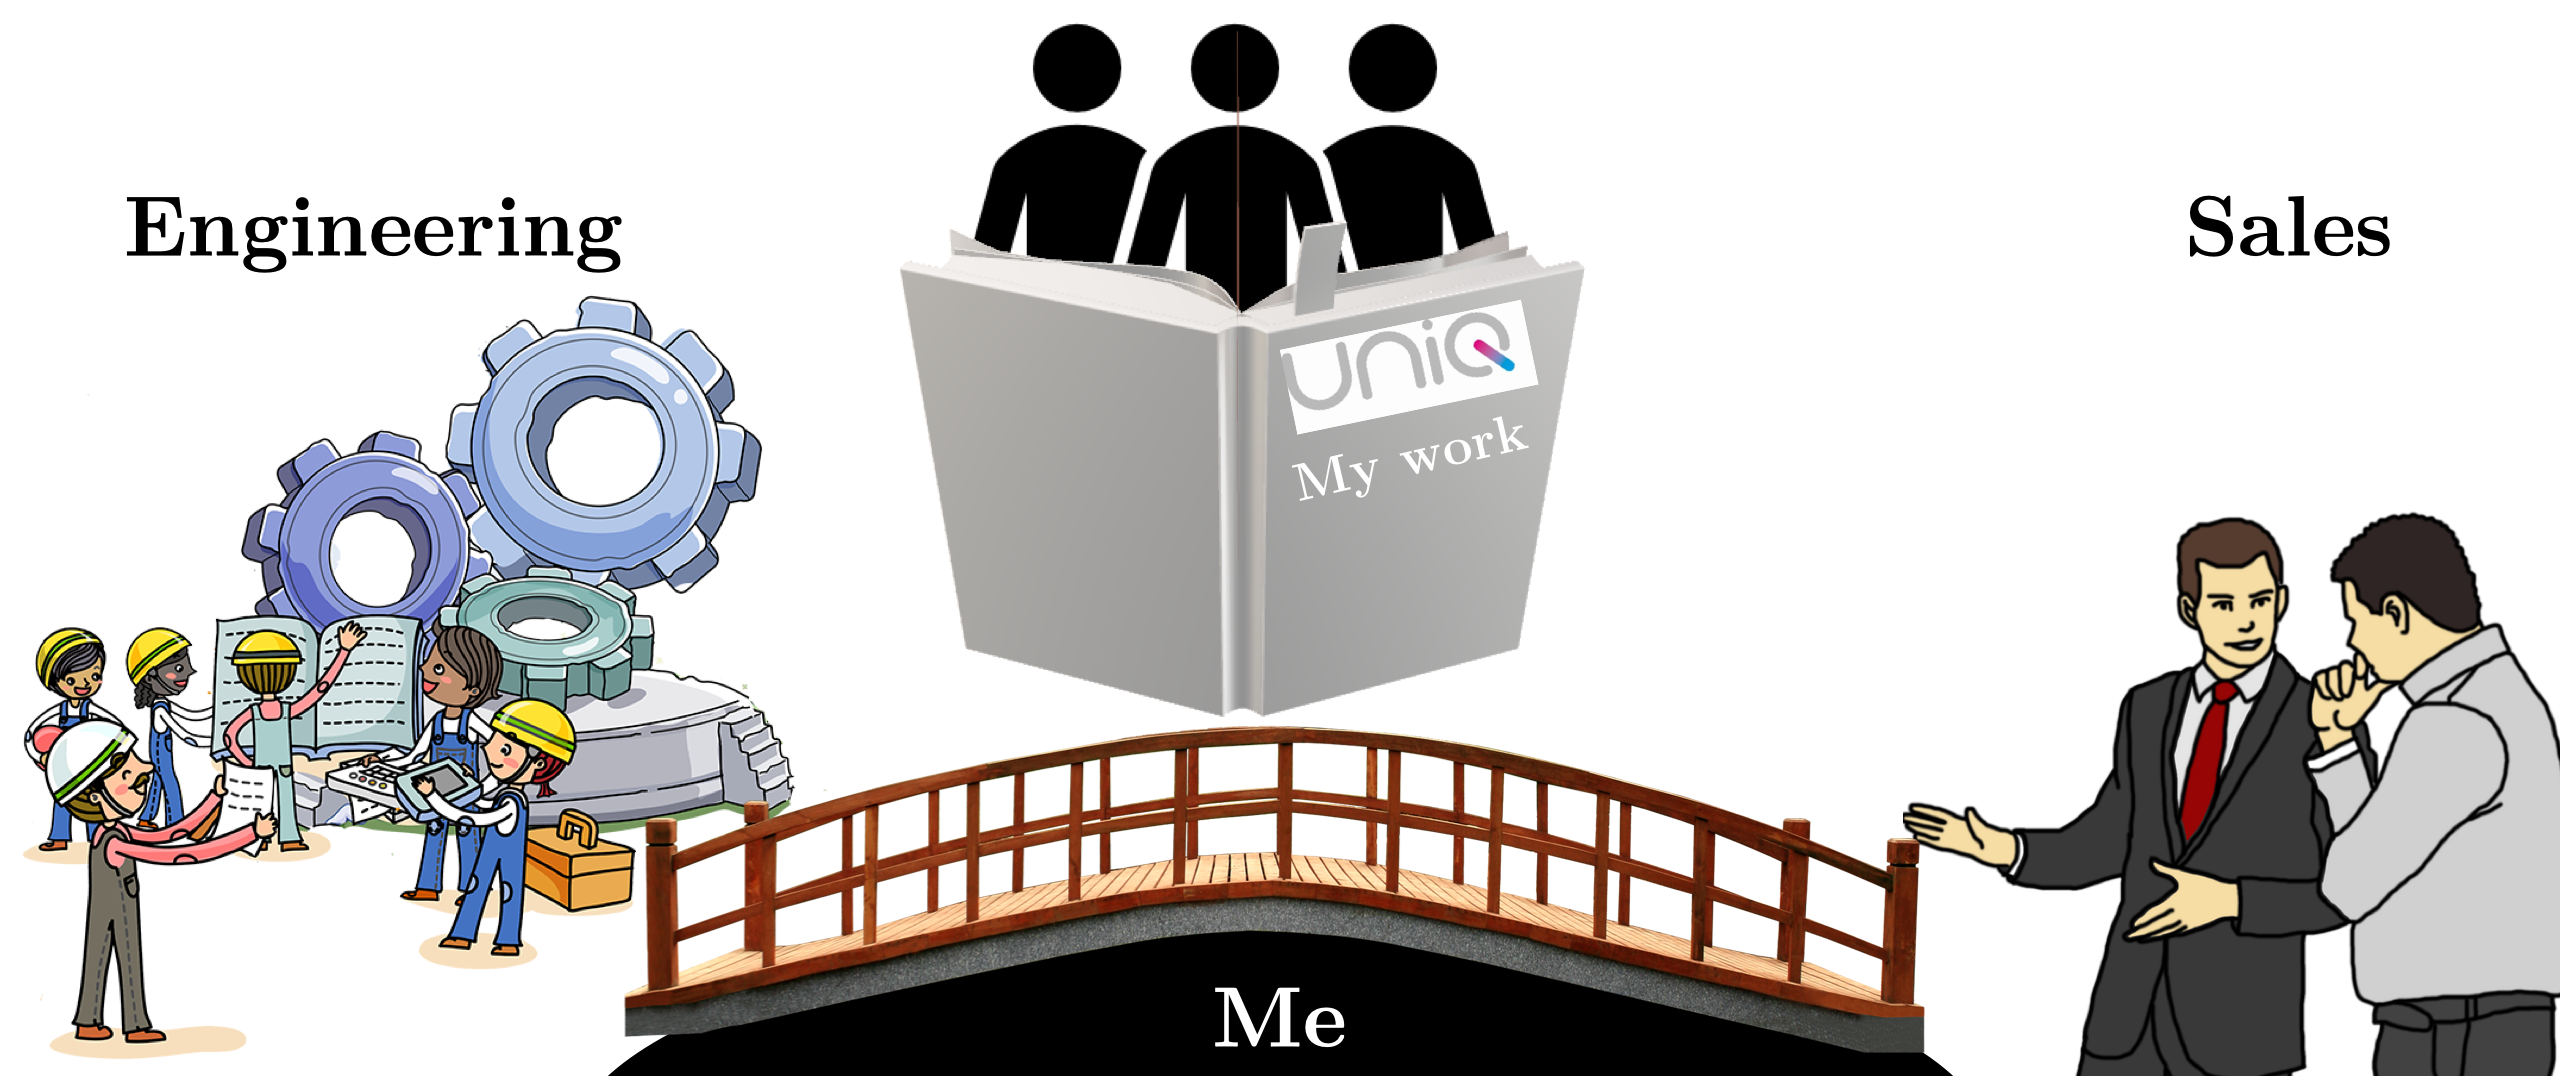
\includegraphics[width=0.4\textwidth]{figures/bridge.png}
	\rule{0.4\textwidth}{0.5pt} % use line???
	\caption{My place at Sunamp.}
	\label{fig:bridge}
\end{wrapfigure}

My placement at Sunamp started on Tuesday 3\textsuperscript{rd} July 2018 and ended on Friday 10\textsuperscript{th} August 2018.
I worked a total of 198 hours across six weeks, averaging at about 6.8 hours of work per day (see log in Appendix~\ref{App:Log}).

I joined Sunamp in the wake of the development of UniQ.
UniQ had been developed by Sunamp's engineers and explained in a manual.
However, the manual was too large and technical for the sales team to understand, navigate and use to efficiently match customers with the most suitable UniQ products.
Therefore, my purpose at Sunamp was to bridge the gap between Engineering and Sales (see Figure~\ref{fig:bridge}).
This was to be done by creating concise and user-friendly documentation that would introduce and explain the UniQ range to customers and even be used by the sales team as an aide-memoire.
This project mainly consisted of me presenting existing content in new ways and boiling down a lot of technical documentation/ material into meaningful and useful information for customers.

My time at Sunamp can roughly be divided up into two aspects: learning about Sunamp's work and development, and
% \hl{producing work for Sunamp/ }
carrying out my UniQ project.




%-----------------------------------
%	SUBSECTION 1
%-----------------------------------

\subsection{Learning About Sunamp}

The majority of my first week at Sunamp consisted of my familiarisation with the company and their products.
The week started with an induction from Susan Lang-Bissell, the Chief Operation Officer (COO), where we went over my contract, office information, health and safety regulations (amongst other things) and I got a brief tour of the factory.
The induction was followed by an introduction from Joan Pisanek (the Business Development Manager) to UniQ and some of Sunamp's projects.
I used the rest of the week to familiarise myself with and try to understand their products by consulting Joan's PowerPoint presentations and the UniQ manuals,
% working through Joan's Buchlyvie project (\hl{see Appendix ...}),
and attempting a UniQ Product Training Exercise developed by Sandy.

Santokh Gataora, colloquially known as Sandy, is Sunamp's Technical Director.
He has a vast experience in building services engineering and has helped develop the UniQ product range.
He writes and continues to refine the UniQ manuals as he guides the company in the engineering and application aspects of UniQ heat batteries in buildings.
% When I joined the company, UniQ was a very recent development that the sales team was still learning about.
% The week I arrived at Sunamp, Sandy had sent out an exercise for the sales team to complete for the following week's UniQ Product Training Workshop.
% The exercise instructions and my answer \hl{can be found in Appendix ... blur out people's names in email}.
During my second week, I attended the UniQ Product Training Workshop, where the sales team and I learned about the UniQ product range in greater depth and briefly went over the solution to the aforementioned exercise.
%\hl{Comment on my answer vs. solution?}

During my second and third weeks at Sunamp, I received more thorough tours of the factory, workshop and chemistry laboratory.
At the factory I got an understanding of the construction of the heat batteries.
I touched a heat battery that had been assembled some days before and left to cool off; it was \emph{still warm} -- I was amazed by its impressively low heat losses!

During the workshop and laboratory tour, I gained a deeper understanding of the making and performance of the PCMs and the selection of materials that go inside a heat battery.
Some of the things I learned are:
\begin{itemize}
    \item The high energy density of the PCMs is what allows Sunamp's heat batteries to be between two and four times smaller than their equivalent hot water cylinders.
    \item Sunamp's chemists cycle and analyse PCM mixtures through solid-liquid and liquid-solid phase transitions to assess the stability of the mixtures' phase transitions over time. The more stable the transitions are, the more suitable they are to be used in heat batteries.
    %\item The chemists also need to test their supplier's materials for impurities which can significantly degrade the performance of PCM mixtures.
    \item Different PCM mixtures can react differently to aluminium and copper, the main metals that heat exchangers are built from.
    Sunamp typically uses all-aluminium finned-tube heat exchangers, but they will sometimes create a PCM which corrodes aluminium.
    In these cases they might need to consider using copper-based heat exchangers, which are more expensive but might work out cheaper in the long-run when compared to the capital and operational costs of the heat batteries' equivalent hot water cylinders.
    \hl{just refer back to your temperature chart and it will make sense and be less alarming}
    %\item Working with cold, medium and high temperature ranges, the chemists need to ensure that the plastic material of the container which holds the PCM can tolerate that PCM's temperature range. Therefore Sunamp typically uses different materials for containers that carry cold and warm/ hot PCMs.
\end{itemize}

During my fourth and fifth weeks at Sunamp, I attended two presentations.
The first was a summary of the research carried out by two chemistry students that had spent the past year working on their dissertation projects at Sunamp.
I gained some insight into the technical aspects of the development of PCMs and was impressed that one of the student's PCMs might soon become patented and used for refrigeration in vehicles.
Sandy gave the second presentation which was an overview of the new UniQ product range to the whole company.
I think this was especially insightful for the chemists and engineers who are specialised in their specific areas and might not always see how all of their work contributes to the end-product (heat batteries) and their application (heating space and water in buildings).

During my last week, I was part of the tour and planning of Sunamp's Experience Room.
This room is designed to look and feel like a home, with a kitchen-like decor and sink in one corner.
One of the purposes of this room, which was still under construction, is to showcase Sunamp's heat batteries to customers by comparing them to their large equivalents on the common marketplace (e.g. hot water cylinders) and by showing how they integrate into a building and its systems (e.g. heat pumps
and boilers).
The room is also planned to be used for training workshops on the installation of Sunamp's heat batteries.

Throughout my brief placement at Sunamp, there has been a sense of rapid development and expansion.
The company started out by manufacturing batteries inside a small workshop, which has now grown into a factory which is still evolving with the construction of new testing facilities and training/ marketing spaces.
The company continues to recruit more engineers and scientists.
It also seems like more customers are hearing about and taking interest in Sunamp's heat batteries, in the UK and abroad.

%\hl{See notebook notes on how to demonstrate technical understanding.}




%-----------------------------------
%	SUBSECTION 2
%-----------------------------------

\subsection{My UniQ Project} \label{sec:sunamp_work}

%\hl{Decide on section title!}

% Ohhhh come on! I gotta write! Just blow off some steam. It doesn't have to be all thought out and structured to begin with. Just keep the hand on the keyboard and type! As Moira says, "Be confident." :D

I started working on my project during my second week at Sunamp and completed it during my last week.
From my log, I have deducted that I worked at least 138 hours on this project, which accounts for 70\% of my time at Sunamp.
This includes the time I spent working autonomously, in meetings, and my final presentation.

I ended up creating a series of documents about UniQ, most of which are illustrated in Figure~\ref{funnel}.
The documents formed a hierarchy, from very generic information at the top to more specific information going down.
This funneling of information reflects the customer's journey, from the time they become aware of a product until they decide to purchase it.
\hlc[cyan]{
When I was preparing for my presentation, I discovered that my funnel resembles a marketing strategy/ concept called the marketing funnel.
This starts out by making customers aware of the product and then increasingly provides more specific information as a customer becomes more interested until they decide to purchase the product.}
\hlc[green]{On reflection...
This corroborated/ validated my use of the funnel.}
At the top of the funnel were documents that introduced and gave an overview of the UniQ product range.
These consisted of the Overview Sheet and UniQ Product Selection Quiz.
At the next level of the funnel were documents that provided specific information about the individual UniQ products; these were called the Product Information Sheets (PISs).
At the bottom of the funnel was a document that provided installation guidelines for the UniQ batteries.


\begin{figure}[htbp]
	\centering
	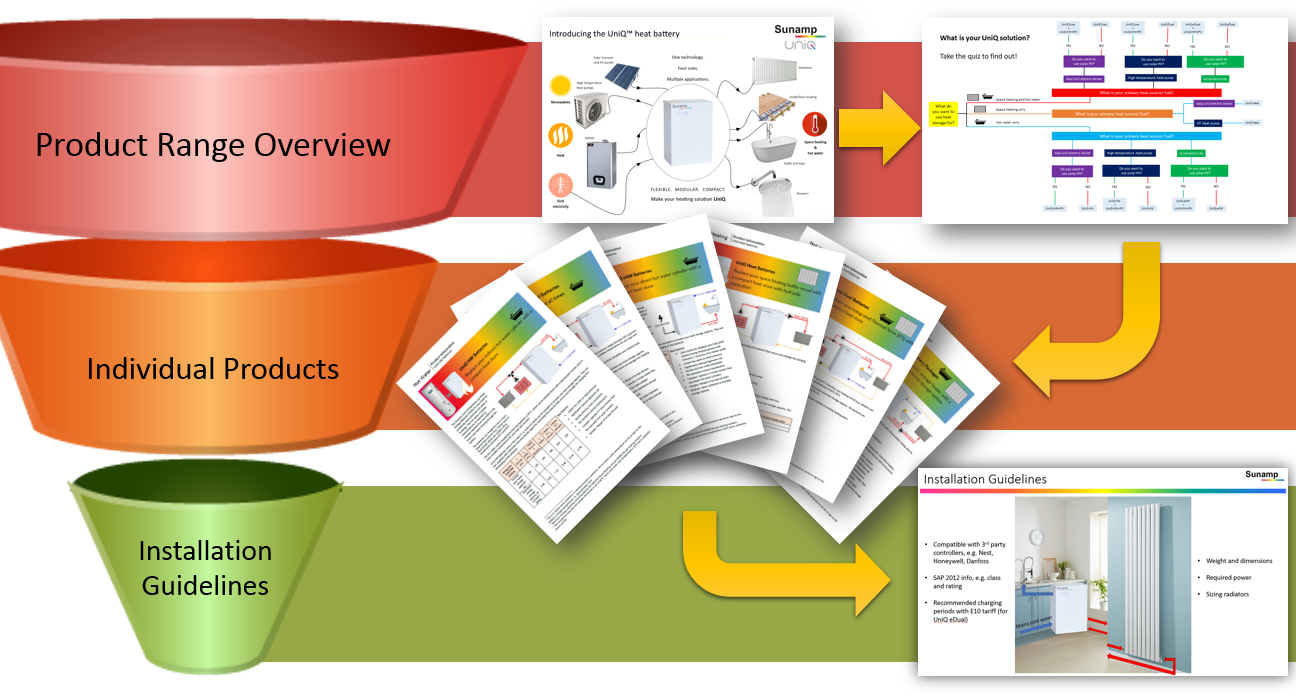
\includegraphics[width=\textwidth]{figures/Funnel.PNG}
	\rule{\textwidth}{0.5pt} % use line???
	\caption{The main outcomes of my UniQ project, ranked by a funnel-shaped hierarchy.}
	\label{funnel}
\end{figure}


Outside the heart of my project, embodied by the information funnel in Figure~\ref{funnel}, I carried out a couple other tasks.
Among these was \hl{a document} I produced that contained additional information that was to be included in Sunamp's upcoming UniQ brochure.
Also, at the end of my placement, I gave a presentation to Sunamp's core staff, including the CEO, about my placement work.

The following sections will discuss my work in more detail.



\subsubsection{UniQ Overview Sheet}

I had not been asked to create a sheet that gave an overview of the UniQ product range.
I, however, thought it might be helpful to ease the customers' introduction to and understanding of UniQ.
The final Overview Sheet (see Appendix~\ref{App:Overview}) introduces the UniQ battery by showing the possible inputs (renewables, heat and/ or electricity) and outputs (space heating and/ or hot water).
The battery is flexible when it comes to its inputs: these can range from boilers to heat pumps, and from grid electricity to PV panels.
Furthermore, the sheet features some catchy ways to describe UniQ, including the tag line ``Make your heating solution UniQ", that I came up with.
\hlc[green]{On reflection, the sheet misses the point of getting a heat battery. Why would I get a battery if I already have the means to generate space heating and hot water. I think this was raised during the meeting by Andrew and was to be rectified after I left.}

It turned out that Sunamp already had a diagram showing the inputs and outputs of a UniQ battery.
However, the staff considered using mine over their original diagram in the UniQ brochure.



\subsubsection{UniQ Product Selection Quiz} \label{sec:quiz}

As I was working on the PISs, the question of how a customer would know which UniQ product was most suitable to them \hl{loomed} in my mind.
``How will they even know which PIS to read?"
That is when I thought of creating a quiz in the form of a decision tree that would ask customers questions and guide them to the most suitable UniQ product for them based on their answers.
An added benefit of the quiz was that it would allow customers to explore the UniQ range easier and more informed, which would cut some of the sales team's initial \hl{customer-product match-making/ interface work}.

Figure~\ref{fig:quiz_draft} shows my first draft of the quiz.
I showed this to Joan when I pitched the quiz idea to her.
The idea was well received by her and Susan, so it escalated to another one of my sub-projects.
After creating a more polished second draft, I asked Sandy to give his expert feedback.
He responded with a re-arranged and more sophisticated decision tree.
This was the start of a process of iterations where I asked staff members for further feedback in order to refine the quiz design.
The full-sized version of the final quiz (Figure~\ref{fig:quiz_final}) can been found in Appendix~\ref{App:quiz}.


%\begin{figure}[htbp]
%	\centering
%	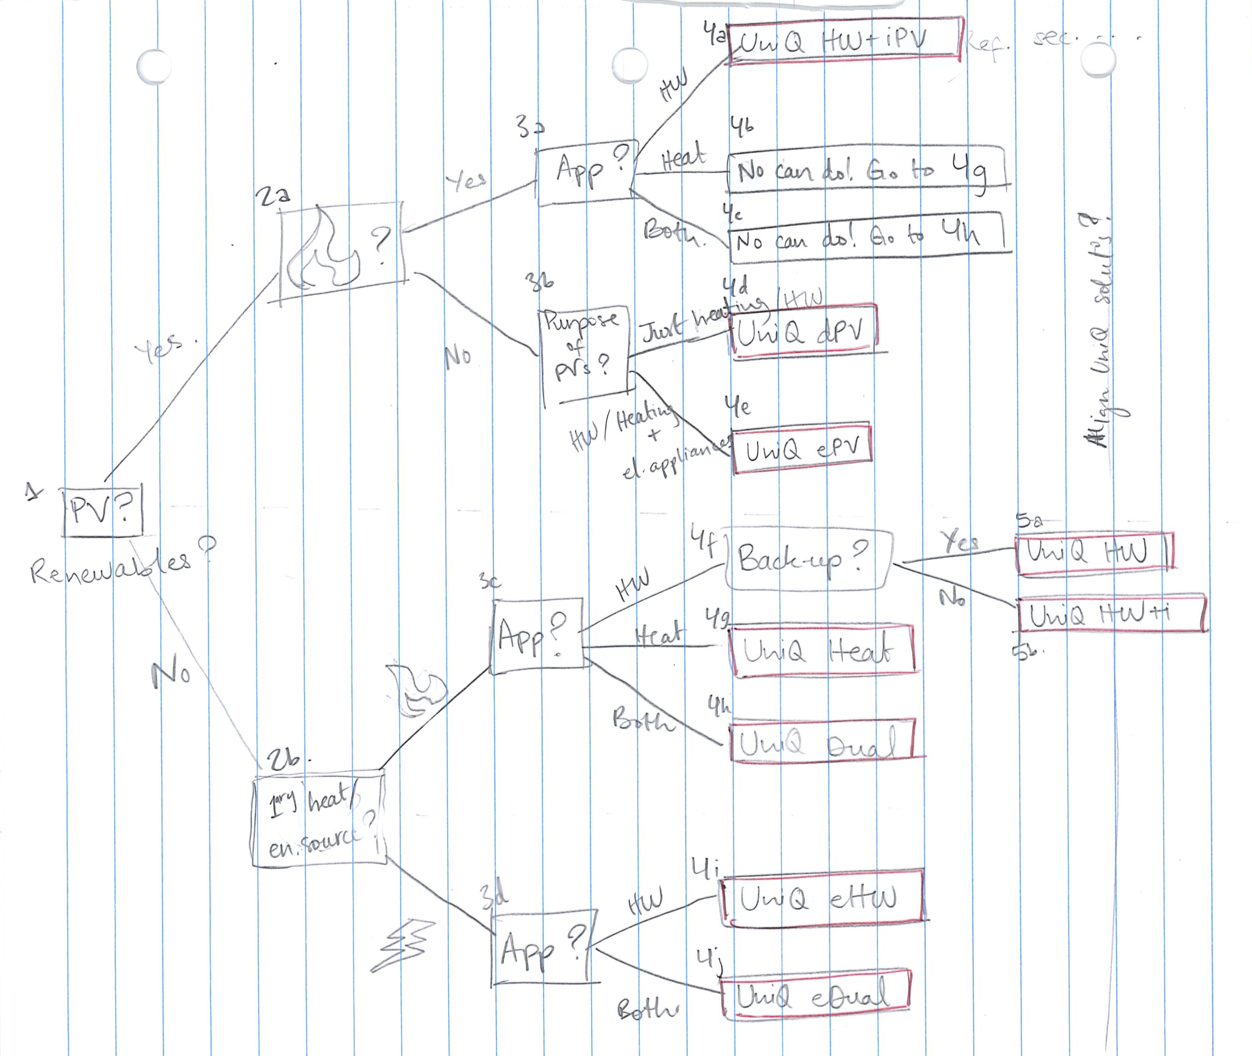
\includegraphics[width=0.5\textwidth]{figures/QuizSketch.png}
%	\rule{\textwidth}{0.5pt} % use line???
%	\caption{My first draft of the UniQ Product Selection Quiz.}
%	\label{quiz_draft}
%\end{figure}


\begin{figure}[htbp]
    \centering
        \begin{subfigure}{.38\textwidth}
          \centering
          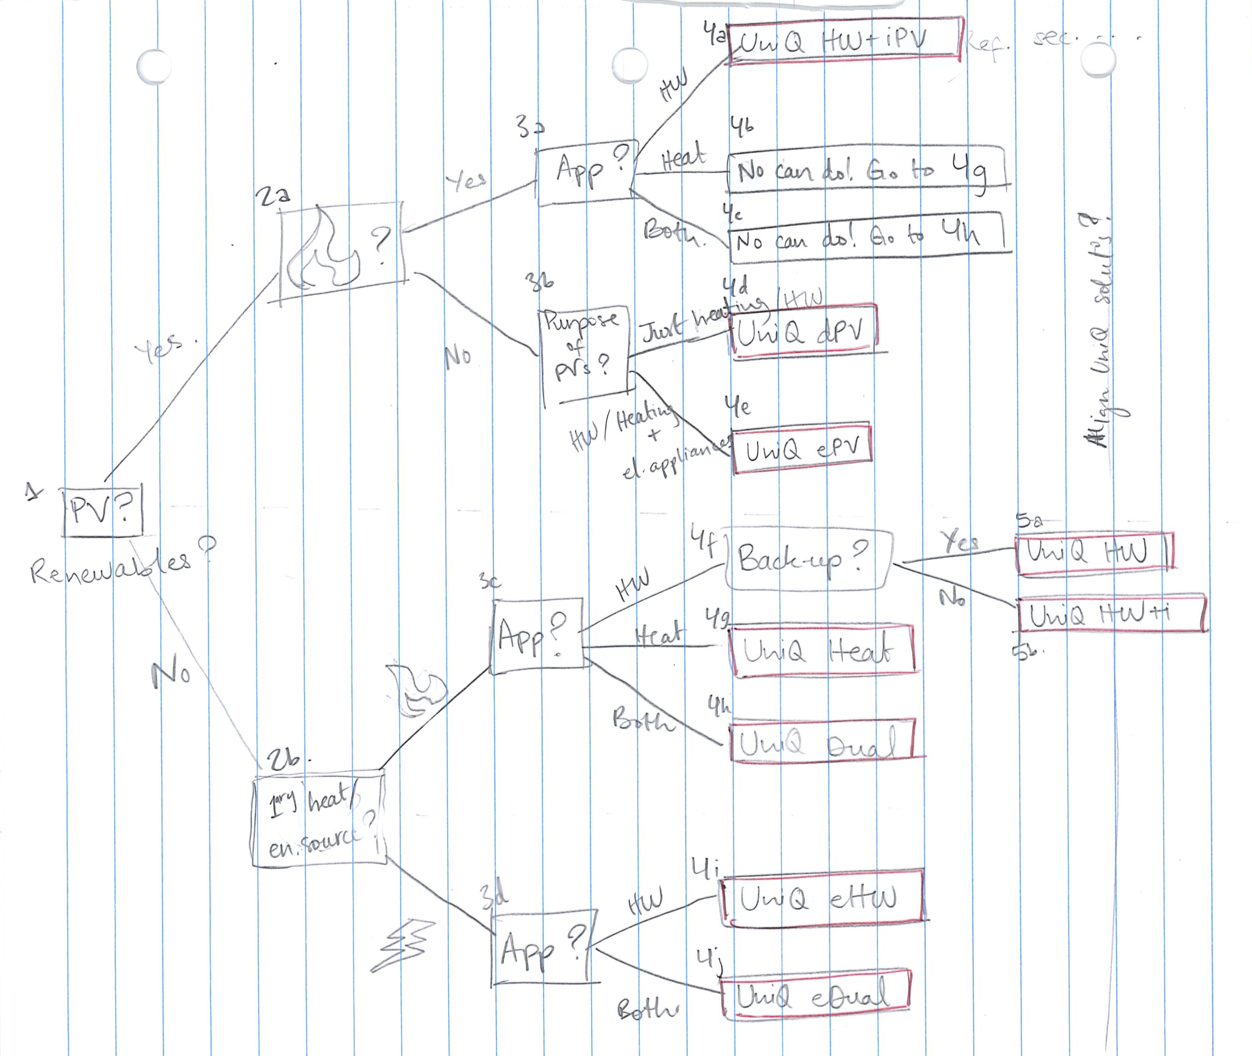
\includegraphics[width=\textwidth]{figures/QuizSketch.png}
%          \rule{\textwidth}{0.5pt} % use line???
          \caption{First draft}
          \label{fig:quiz_draft}
        \end{subfigure}
        \begin{subfigure}{.58\textwidth}
          \centering
          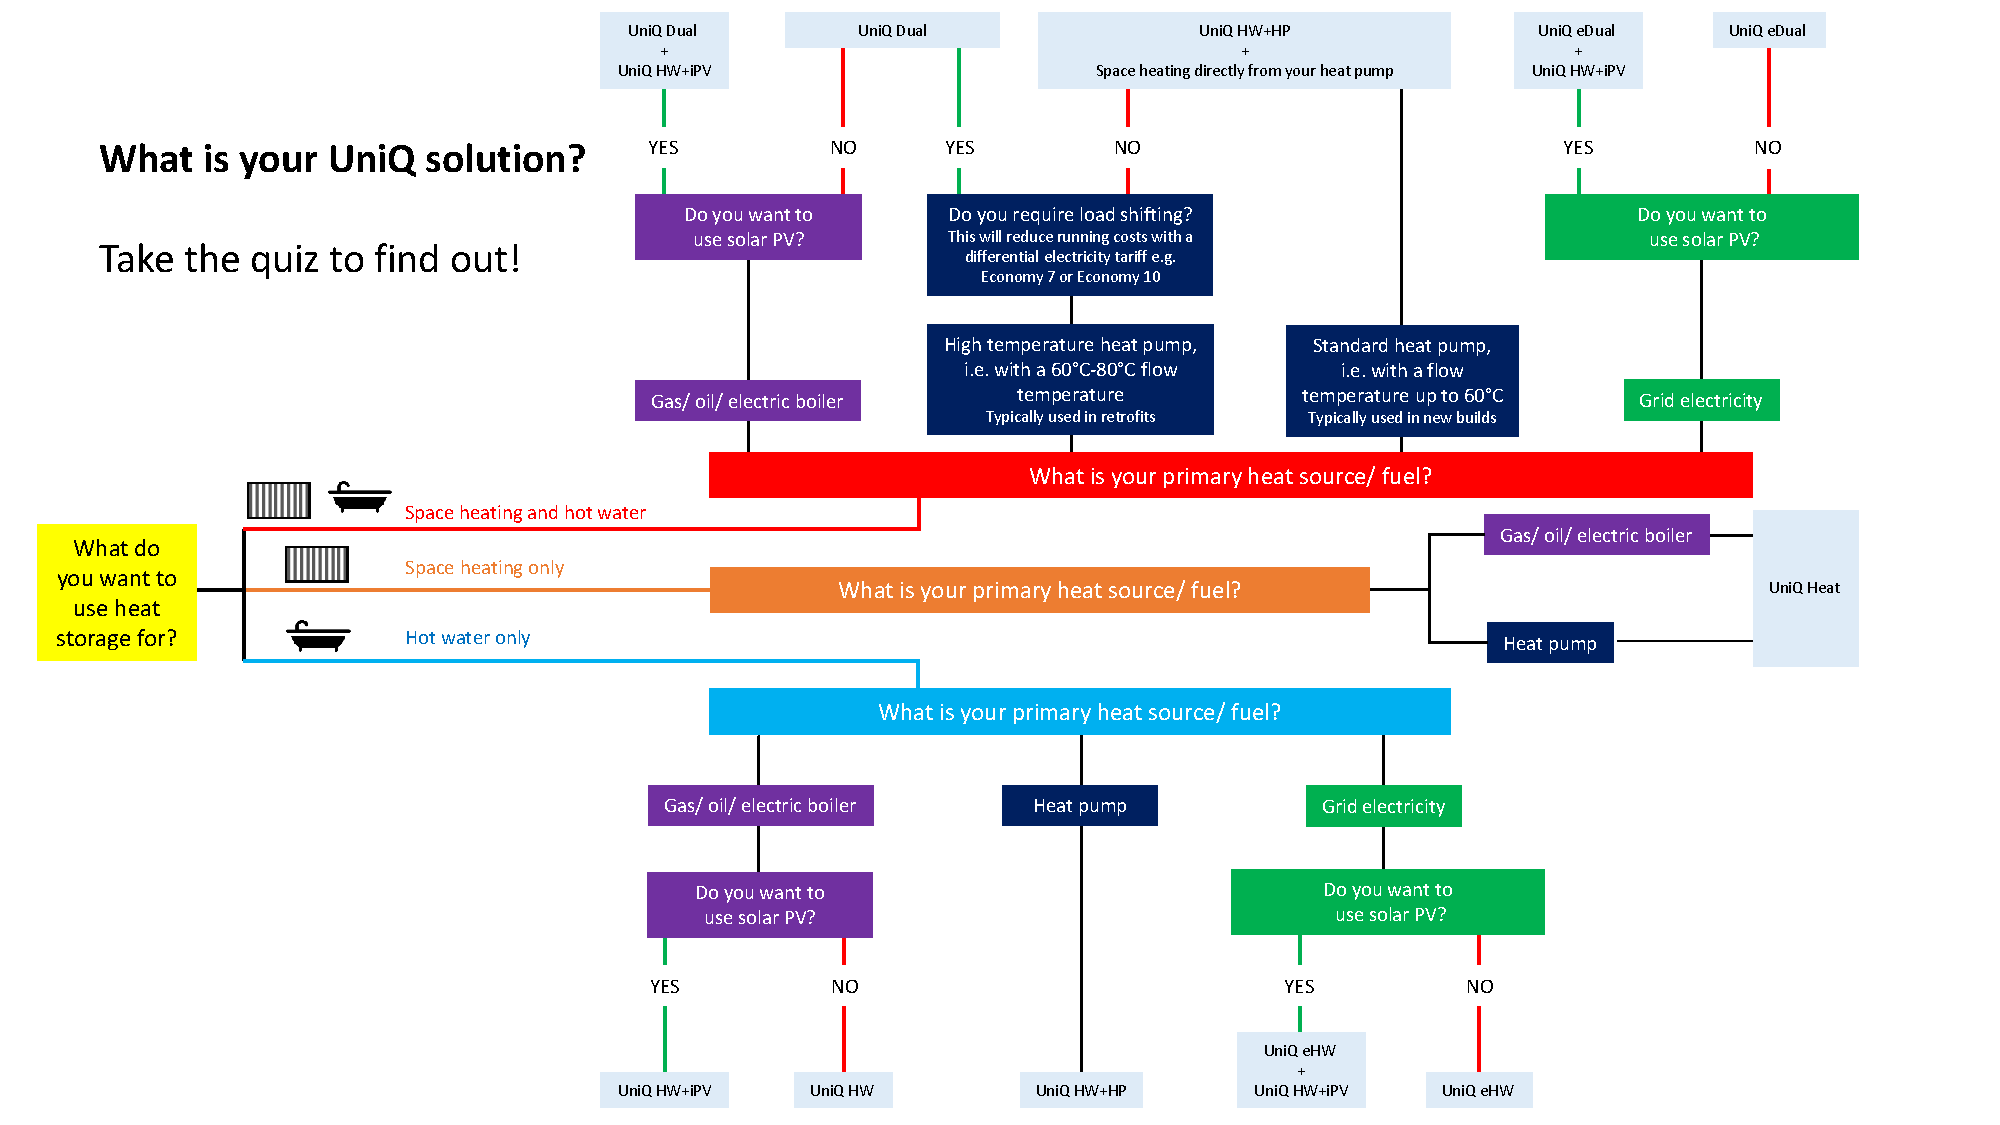
\includegraphics[width=\textwidth]{Appendices/final_quiz.pdf}
%          \rule{\textwidth}{0.5pt} % use line???
          \caption{Final result}
          \label{fig:quiz_final}
        \end{subfigure}
    \rule{\textwidth}{0.5pt} % use line???
    \caption{The first draft and final result of the UniQ Product Selection Quiz.}
    \label{fig:quiz}
\end{figure}



\subsubsection{UniQ Product Information Sheets (PISs)} \label{sec:piss}

Sandy asked me to produce a PIS for each of the UniQ products.
He gave me an outline of the type of information that would be included on each sheet, e.g. a brief description of the product and its operation, a diagram, and battery sizing information.
%, hydraulic connections, a wiring diagram, and a ``Do's and Don'ts!" list.
Every PIS was limited to two sides of an A4 page.

\begin{wrapfigure}{r}{0.4\textwidth}
	\centering
	\begin{subfigure}{.19\textwidth}
		\centering
		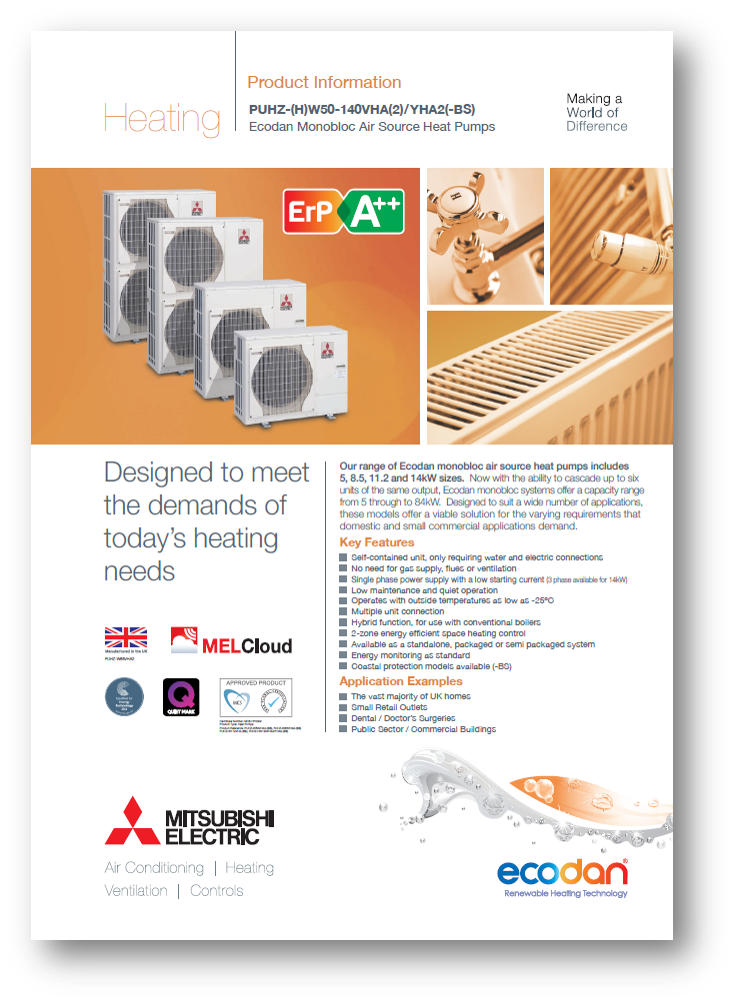
\includegraphics[width=\textwidth]{figures/Mitsubishi01.png}
		%          \rule{\textwidth}{0.5pt} % use line???
		\caption{Front}
		\label{mitsubishi01}
	\end{subfigure}
	\begin{subfigure}{.19\textwidth}
		\centering
		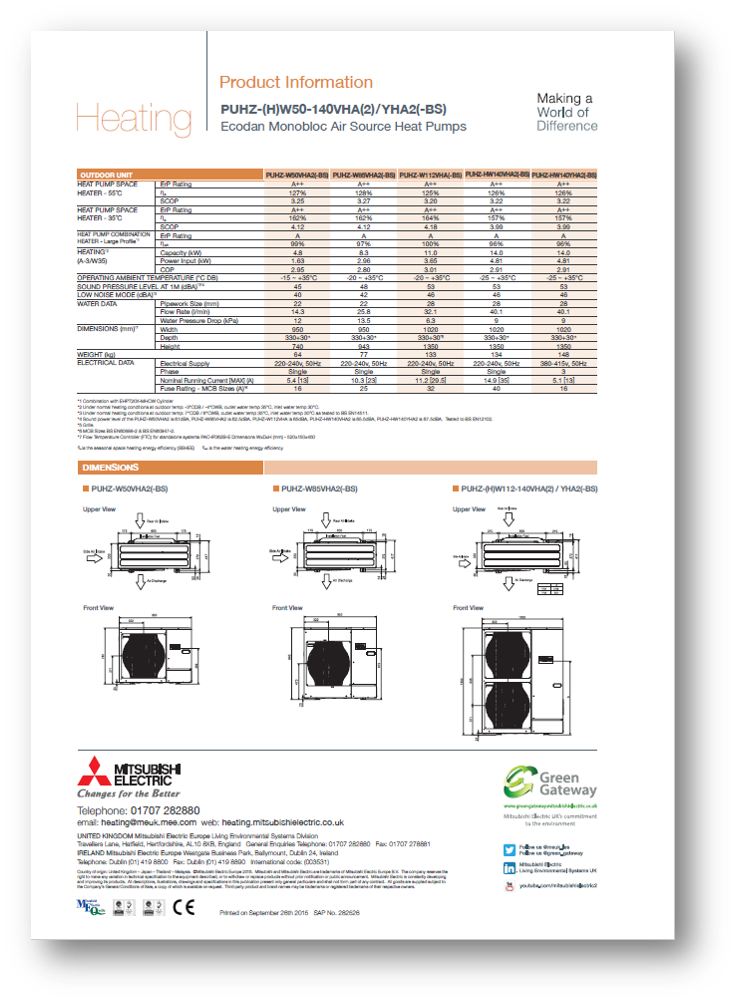
\includegraphics[width=\textwidth]{figures/Mitsubishi02.png}
		%          \rule{\textwidth}{0.5pt} % use line???
		\caption{Back}
		\label{mitsubishi02}
	\end{subfigure}
	\rule{0.4\textwidth}{0.5pt} % use line???
	\caption[Mitsubishi's PISs.]{One of Mitsubishi's PISs that I drew inspiration from \citep{ref:Mitsubishi}.}
	\label{mitsubishi}
\end{wrapfigure}

To accomplish this task, I used a variety of resources.
I obtained the relevant content from Sunamp's UniQ manuals and other documents.
Sometimes, however, the manuals were unclear or contradictory, e.g. regarding the dimensions of the UniQ batteries.
Therefore, to ensure accuracy of the PISs' content, I conducted little investigations e.g. measuring the dimensions of the UniQ batteries in the factory.
For the layout and presentation, I drew inspiration from a couple PISs by Mitsubishi (see one example in Figure~\ref{mitsubishi}).
Similarly to the quiz, the production of the UniQ PISs was a process of iterations where I asked staff members (notably Joan and Sandy) for feedback throughout.
The creation of each UniQ PIS took around ten iterations or more.



During my fifth week at Sunamp, I took part in a meeting with Susan (COO), Joan, Susan Dinwoodie (Executive Personal Assistant), and Maggie Wright (Maggie Wright Associates, a Public Relations company)
who had come into the office to discuss the design of the UniQ brochure.
We discussed incorporating the UniQ Overview Sheet, Product Selection Quiz and PISs in the brochure as well as their possible publication on the website and as flyers.
Since a professional designer would polish the appearance of my work, I was asked to focus more on the content and its accuracy than the presentation.
That is why I have not included the UniQ logo in the PISs, for example.
% on finalising the content and ensuring its accuracy rather than worrying about the presentation.
% Also, other decisions were made, e.g. to remove the hydraulic connections and wiring diagrams.

Before the PISs could be sent to Maggie, they needed to be reviewed and approved by Sandy and, ultimately, Andrew.
By the end of my placement, however, I did not get the opportunity to run the latest versions of the PISs by Andrew or Sandy.
In order to express my uncertainties of these drafts, I left the following message and amended the drafts accordingly:
\begin{itemize}
    \item ``\textcolor{red}{Texts in red} express my uncertainties in their expression or phrasing; these may require amending. This includes all the taglines.
    \item ``I have expressed other uncertainties in comments in the document markups."
\end{itemize}

The UniQ PIS drafts that I left with Sunamp can be found in Appendix~\ref{App:PISs}.
Figure~\ref{breakdown} provides a breakdown of the PISs' structure and layout.



\subsubsection{UniQ Installation \& Operation (I\&O) Sheets}

Joan asked me to create documentation that presented important information that might affect the viability of using UniQ products in a system/ on a project, as well as answers to customers' frequently asked questions (FAQs).
``Will Sunamp install the UniQ battery for me?" and ``How will the UniQ battery integrate into my heating system?" are a couple FAQs, paraphrased.
It turned out that most of these questions were related to the installation and operation of UniQ batteries, hence why I have called them UniQ I\&O Sheets.

%The purpose of the I\&O Sheets was to provide customers with important information when they were considering or ready to purchase a UniQ battery.
Joan wanted the sheets to consist of an annotated floor plan, where one can see where/ how a UniQ battery fits into a home's heating and hot water set-up (see a draft in Appendix~\ref{App:ino}).
I, however, raised the point that a technical architectural drawing like a floor plan might not be easily interpreted by a customer.
I suggested that she may want a sheet with a greater visual impact, as exemplified in Figure~\ref{fig:installation}, or a completely different type of document.
After I started working on the UniQ PISs, Joan considered that the PISs might actually meet her needs better than the I\&O Sheets.
Still, she expressed a desire for the I\&O Sheets to be produced.
I therefore continued to work on the I\&O Sheets but I focused my attention on the PISs.

\begin{figure}[htbp]
	\centering
	\begin{subfigure}{.48\textwidth}
		\centering
		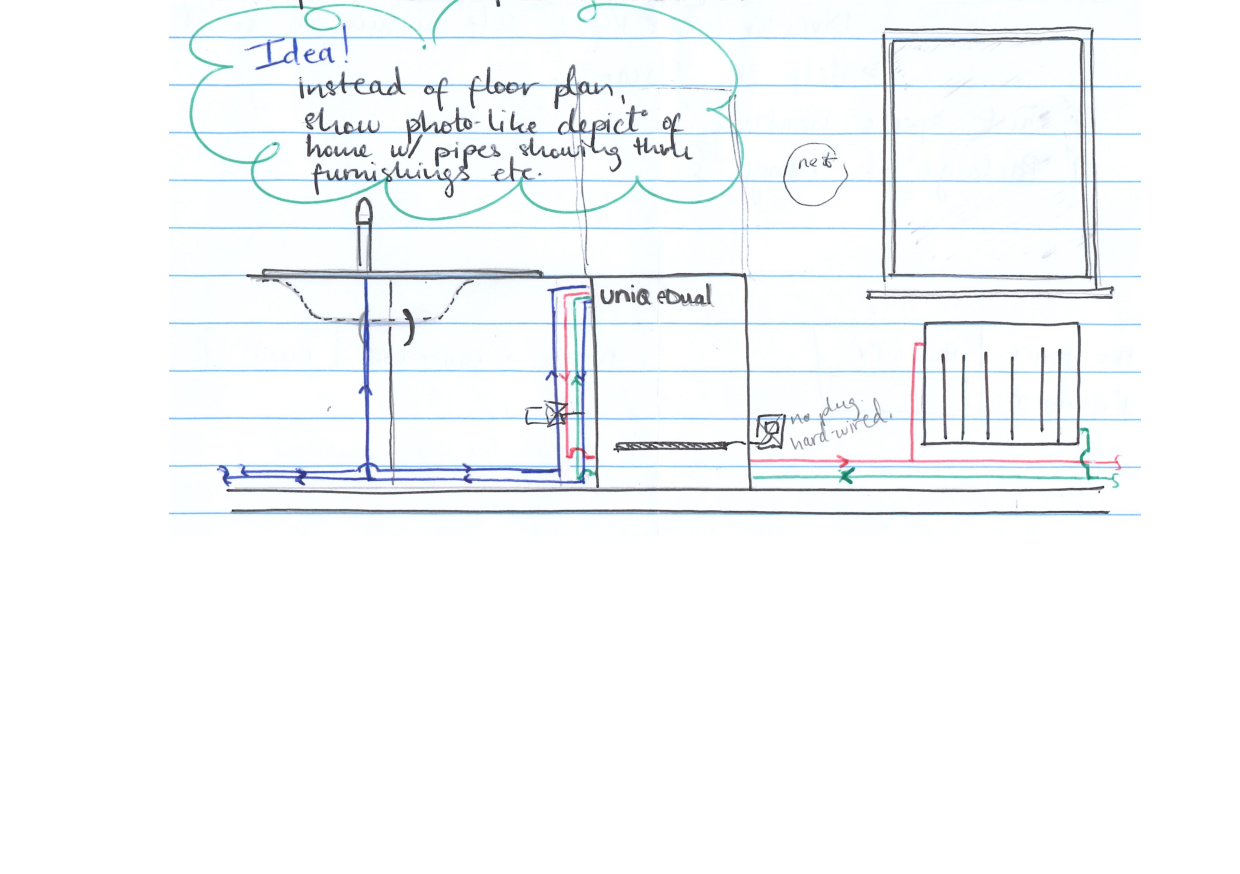
\includegraphics[width=\textwidth]{figures/InstallationSketch.pdf}
		%          \rule{\textwidth}{0.5pt} % use line???
		\caption{Initial sketch of central image}
		\label{fig:installation_sketch}
	\end{subfigure}
	\begin{subfigure}{.48\textwidth}
		\centering
		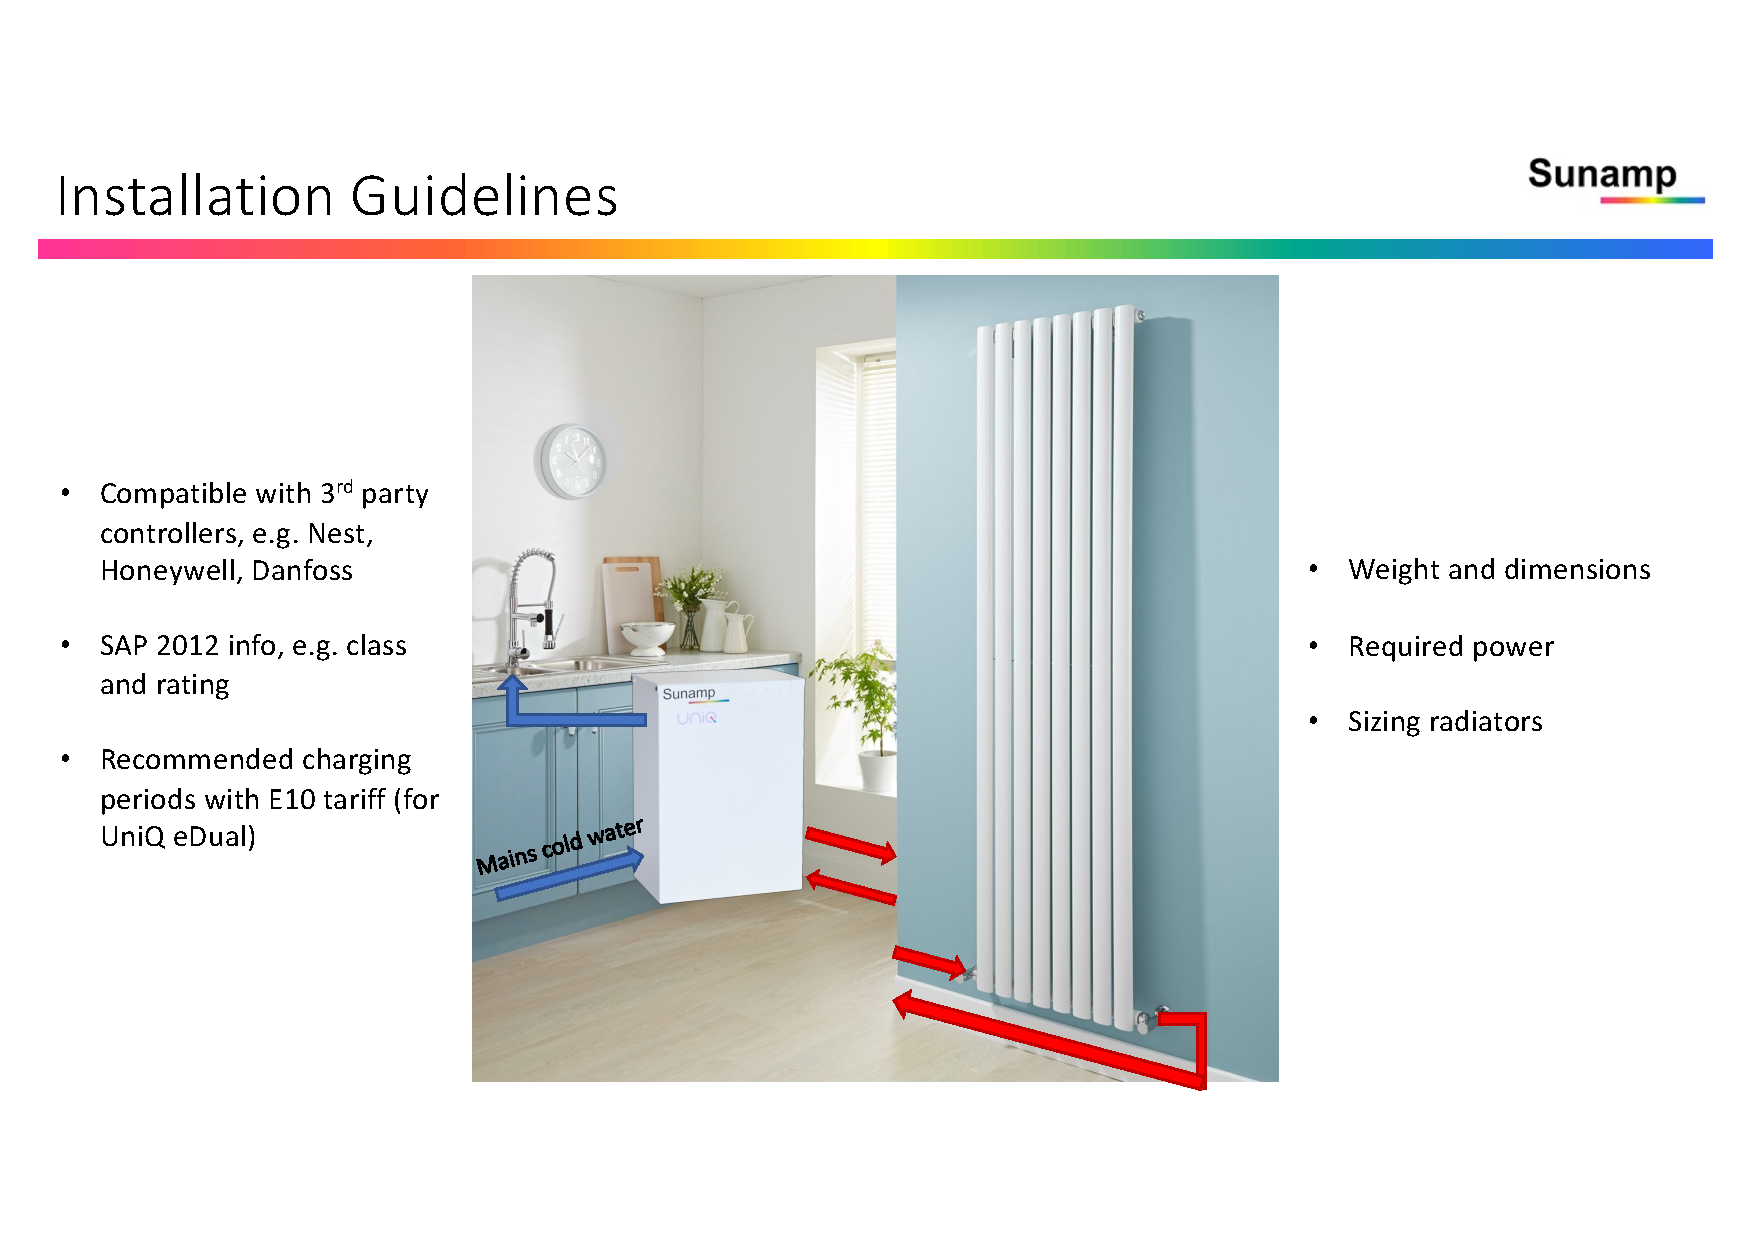
\includegraphics[width=\textwidth]{figures/InstallationGuidelines.pdf}
		%          \rule{\textwidth}{0.5pt} % use line???
		\caption{Draft}
		\label{fig:installation_draft}
	\end{subfigure}
	\rule{\textwidth}{0.5pt} % use line???
	\caption{Drafts of UniQ I\&O Sheets that would have a greater visual impact.}
	\label{fig:installation}
\end{figure}



%\subsubsection{Additional Information for UniQ Brochure}





\subsubsection{Presenting my Placement Work}

During my last week, I gave a 20-minute presentation about the work I had produced to six members of Sunamp's core staff, including Andrew, Susan and Sandy.
(See PowerPoint in Appendix~\ref{App:Presentation}.)
When I presented the UniQ PISs, I gave each staff member a different printed copy of the PISs to examine more closely.
The presentation became quite interactive as I received feedback and we discussed the flow and improvement of the different UniQ documents.
The presentation was a constructive session as it made the core staff (most importantly Andrew) aware of my work and its potential usefulness to the company's marketing.
It was decided that the UniQ I\&O Sheets were not necessary and that some of the information presented on these sheets could be incorporated into the PISs.
The discussion also highlighted some aspects that I had failed to include in the documents by an oversight, notably explaining the interest in storing heat.
I was left with some pointers on last-minute improvements to make on the documents before I left.

\hlc[cyan]{Since I gave my presentation very close to the end of my placement, I did not have time to make all the corrections and improvements that had been highlighted during the presentation.}
\hlc[green]{On reflection, it could have been more constructive to give two presentations (first halfway through the placement and the second at the end) to allow time for me to implement their feedback.}


\begin{figure}[htbp]
	\centering
	\begin{subfigure}{\textwidth}
		\centering
		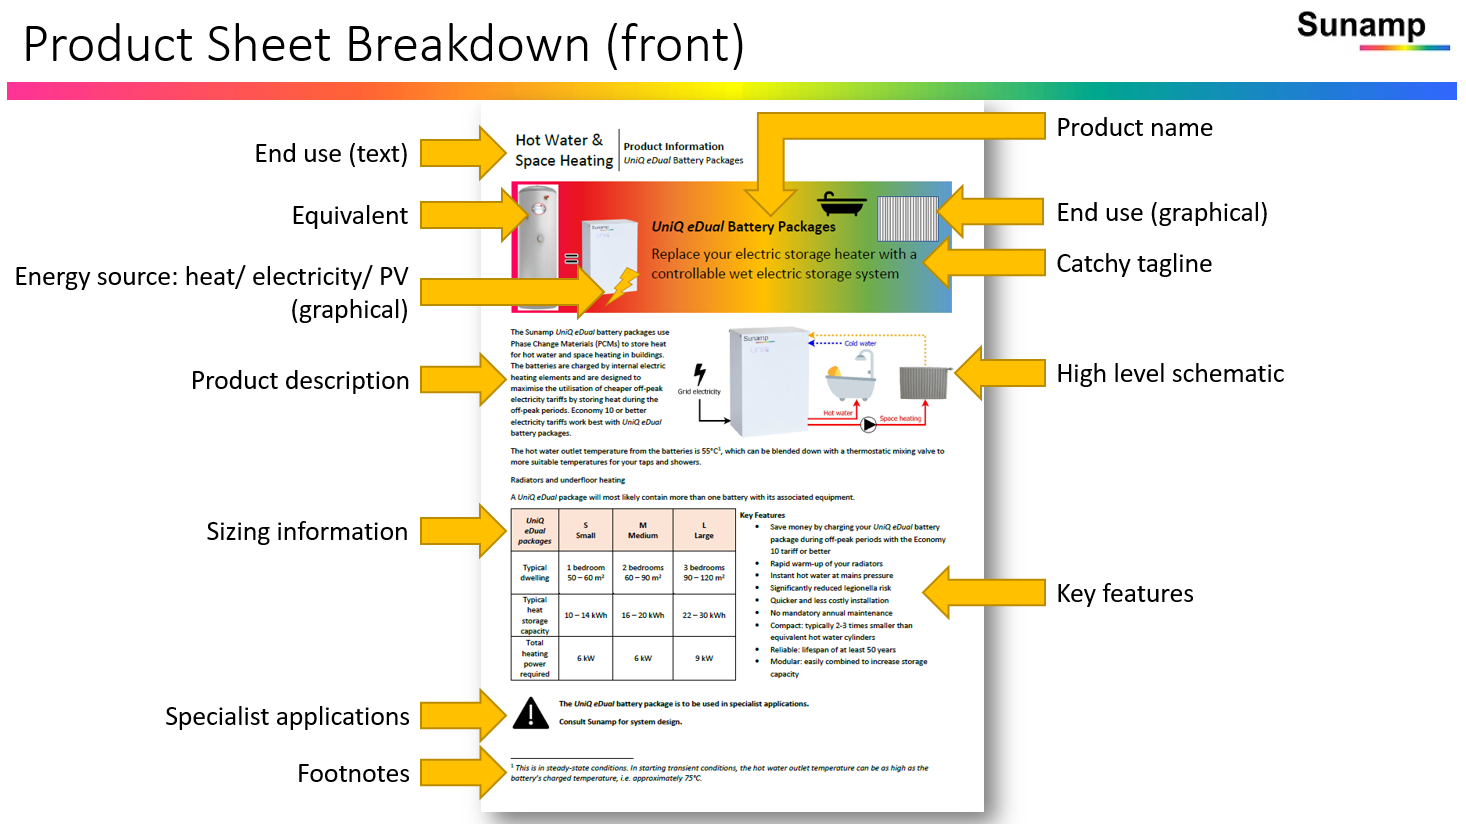
\includegraphics[width=\textwidth]{figures/PIS_breakdown_01.PNG}
		%          \rule{\textwidth}{0.5pt} % use line???
		%          \caption{Front}
		\label{breakdown01}
	\end{subfigure}
	\begin{subfigure}{\textwidth}
		\centering
		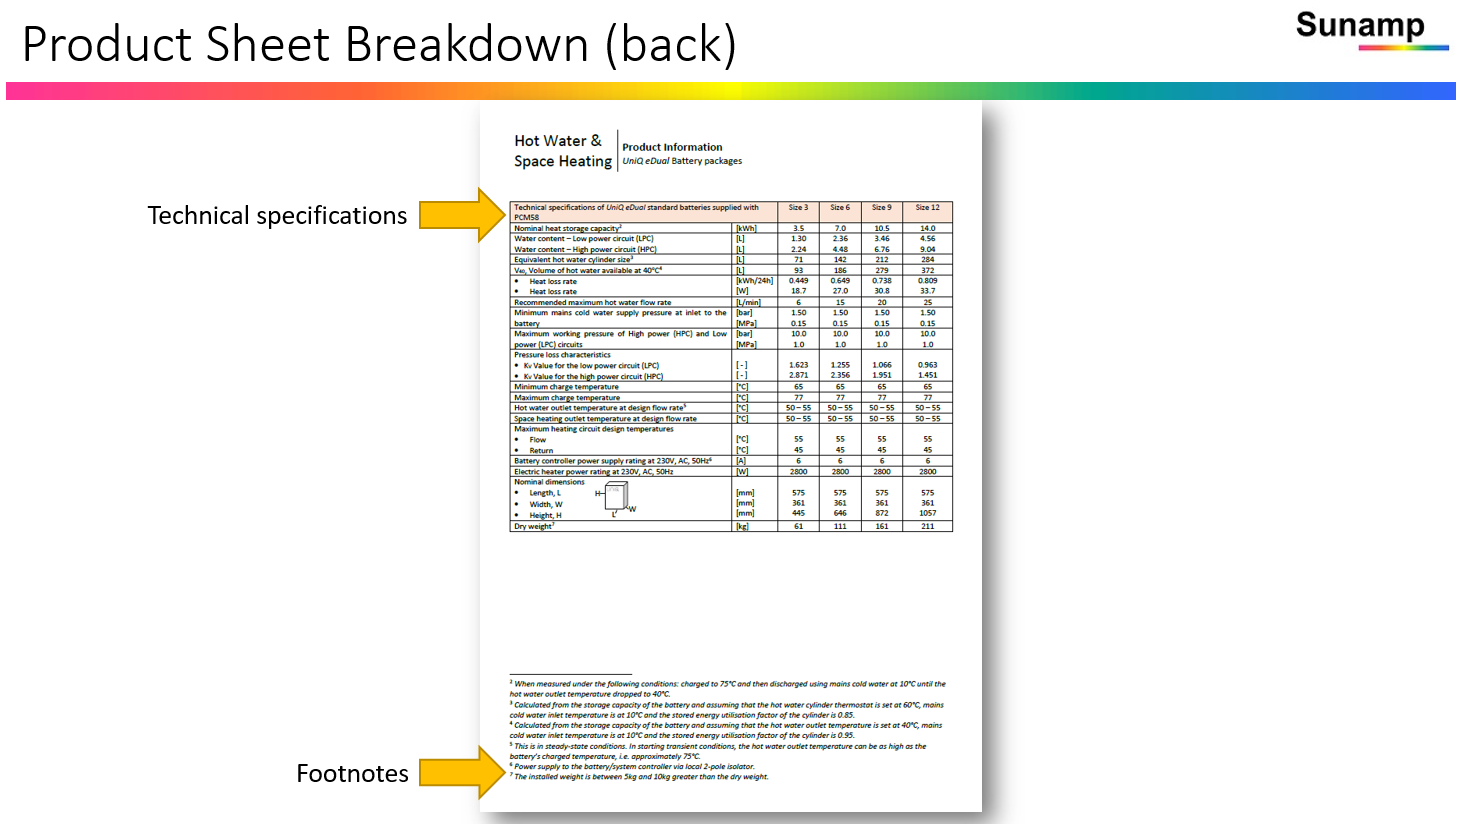
\includegraphics[width=\textwidth]{figures/PIS_breakdown_02.PNG}
		%          \rule{\textwidth}{0.5pt} % use line???
		%          \caption{Back}
		\label{breakdown02}
	\end{subfigure}
	\rule{\textwidth}{0.5pt} % use line???
	\caption{A breakdown of the composition of the UniQ PISs.}
	\label{breakdown}
\end{figure}




\subsubsection{My Contribution to Sunamp}

I contacted Joan and Susan in November 2018 and received an update on how I have contributed to Sunamp.
I was told that my work had not been included in the UniQ brochure because it had to be published quickly, but they are looking to include my material in the next brochure update due after Christmas.
Joan said that she personally used the work that I produced and that it helped her a lot.
Overall, though, Joan said that, ``The biggest legacy of your work here I think is that we now understand what we need in a design team, consisting of people with your experience and recruitment is due to start soon".


